\documentclass[hyperref={pdfpagelabels=false}]{beamer}
\setbeamercolor{block title}{bg=red!30,fg=black}
\usepackage{bm}
\usepackage{lmodern}
\usepackage{amsmath}
\usepackage{centernot}
\usepackage[autostyle]{csquotes}
\usepackage{tikz}
%\usepackage{authblk}
\usepackage{float}
\usetikzlibrary{positioning, calc, shapes.geometric, shapes, shapes.multipart, arrows.meta, arrows, decorations.markings, external, trees}
\usepackage{biblatex}
\addbibresource{Bibliography-MM-MC.bib}

\newlength\myindent
\setlength\myindent{2em}
\newcommand\bindent{%
  \begingroup
  \setlength{\itemindent}{\myindent}
  \addtolength{\algorithmicindent}{\myindent}
}
\newcommand\eindent{\endgroup}

\tikzstyle{Arrow} = [
	thick, 
	decoration={
		markings,
		mark=at position 1 with {
			\arrow[thick]{latex}
			}
		}, 
	shorten >= 3pt, preaction = {decorate}
	]

\usetheme{Frankfurt}
\usepackage[usenames, dvipsnames]{color}
\newcommand{\backupbegin}{
   \newcounter{finalframe}
   \setcounter{finalframe}{\value{framenumber}}
}
\setbeamertemplate{footline}[frame number]

\newcommand{\backupend}{
   \setcounter{framenumber}{\value{finalframe}}
}

\setbeamercovered{dynamic}% see beamer documentation p 190
%\beamerdefaultoverlayspecification{<+>}
\title{The Effect of Medicaid Expansion on Adult Uninsurance Rates: Estimating the Treatment Effect on Non-expansion States}  
%\author{\large{Rahul Ladhania}, \small{CMU} \\ \large{Amelia Haviland}, \small{CMU} \\ \large{Neeraj Sood}, \small{USC} \\ \large{Ateev Mehrotra}, \small{Harvard Medical School}}
\author[shortname]{Max Rubinstein \\}
\institute[]{\and \vspace{-0.26in} \and \vspace{-0.1in}}%\vspace{0ex} 
%\small{Carnegie Mellon University}}
%\subtitle{NBER Machine Learning in Healthcare Meeting}
\date{}

\expandafter\def\expandafter\insertshorttitle\expandafter{%
  \insertshorttitle\hfill%
  \insertframenumber\,/\,\inserttotalframenumber}
  \setbeamertemplate{navigation symbols}{}
  \begin{document}
% \logo{\includegraphics[scale=0.15]{CMU_Logo_Horiz_Red}}

\begin{frame}
\titlepage
\centering 
\vspace{-0.5in}
\textbf{January 19, 2021}
\end{frame} 

\section{Introduction}
\subsection{Background}
\begin{frame}{Background}
\begin{itemize}
    \item Medicaid is a state-administered program that provides health insurance to low-income Americans \bigskip 
    
    \item The 2010 Affordable Care Act mandated that all states expand their eligibility requirements to cover all childless adults up to 138 percent of the federal poverty line (FPL) \bigskip
    
    \item A 2012 Supreme Court ruling made expansion optional for states \bigskip
    
\end{itemize}
\end{frame}

\begin{frame}{Background}
    \begin{center}
	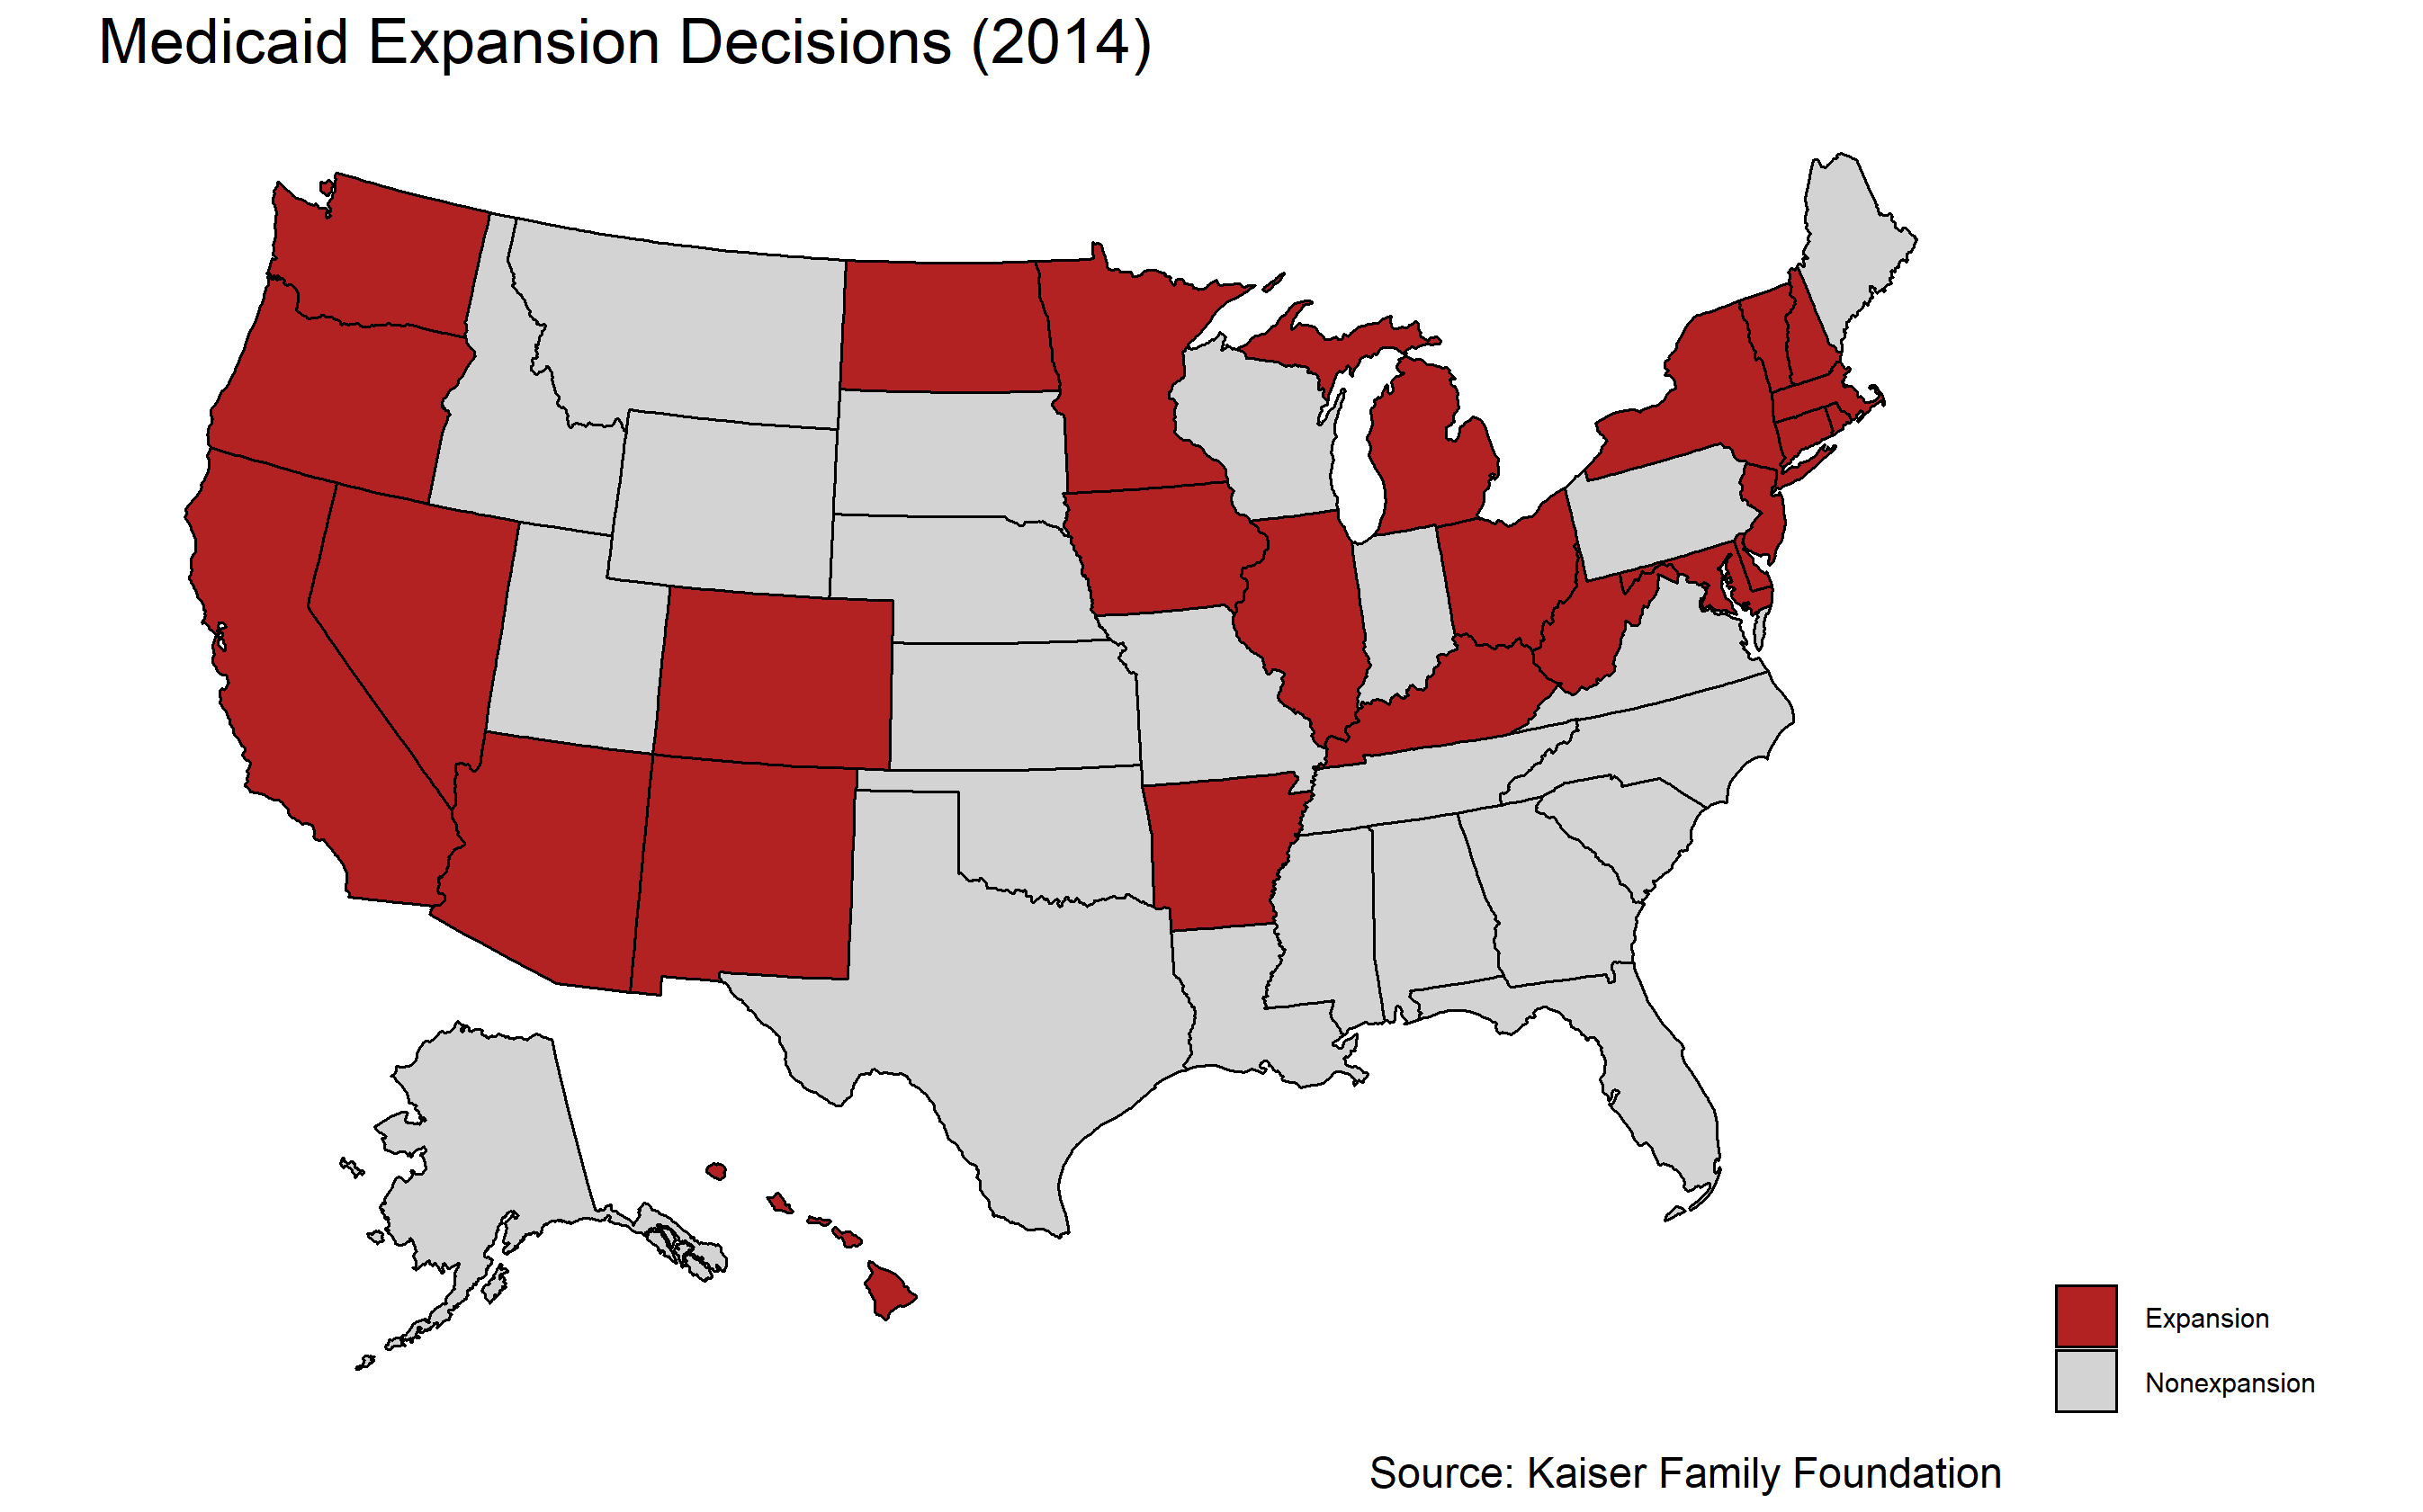
\includegraphics[scale=0.5]{01_Plots/expansion-map.png}
    \end{center}
\end{frame}

\begin{frame}{Motivation}
    \begin{itemize}
    \item Insuring previously uninsured individuals mediates many effects of Medicaid expansion \bigskip
    \item Existing literature primarily targets the ETT; the ETC has rarely been directly studied \bigskip
    \begin{itemize}
        \item Miller et al (2019) predict that 15,000 deaths would have been avoided had non-expansion states expanded Medicaid \bigskip
        \item If treatment effect heterogeneity, we cannot simply use existing estimates of ETT to understand the ETC \bigskip
    \end{itemize}
    \item We believe that the association between governance and Medicaid enrollment would make it likely these effects are smaller in absolute magnitude (see, eg, Sommers (2012)) \bigskip
    \end{itemize} 
\end{frame}

\begin{frame}{State political ideology and Medicaid Expansion}
    \begin{center}
	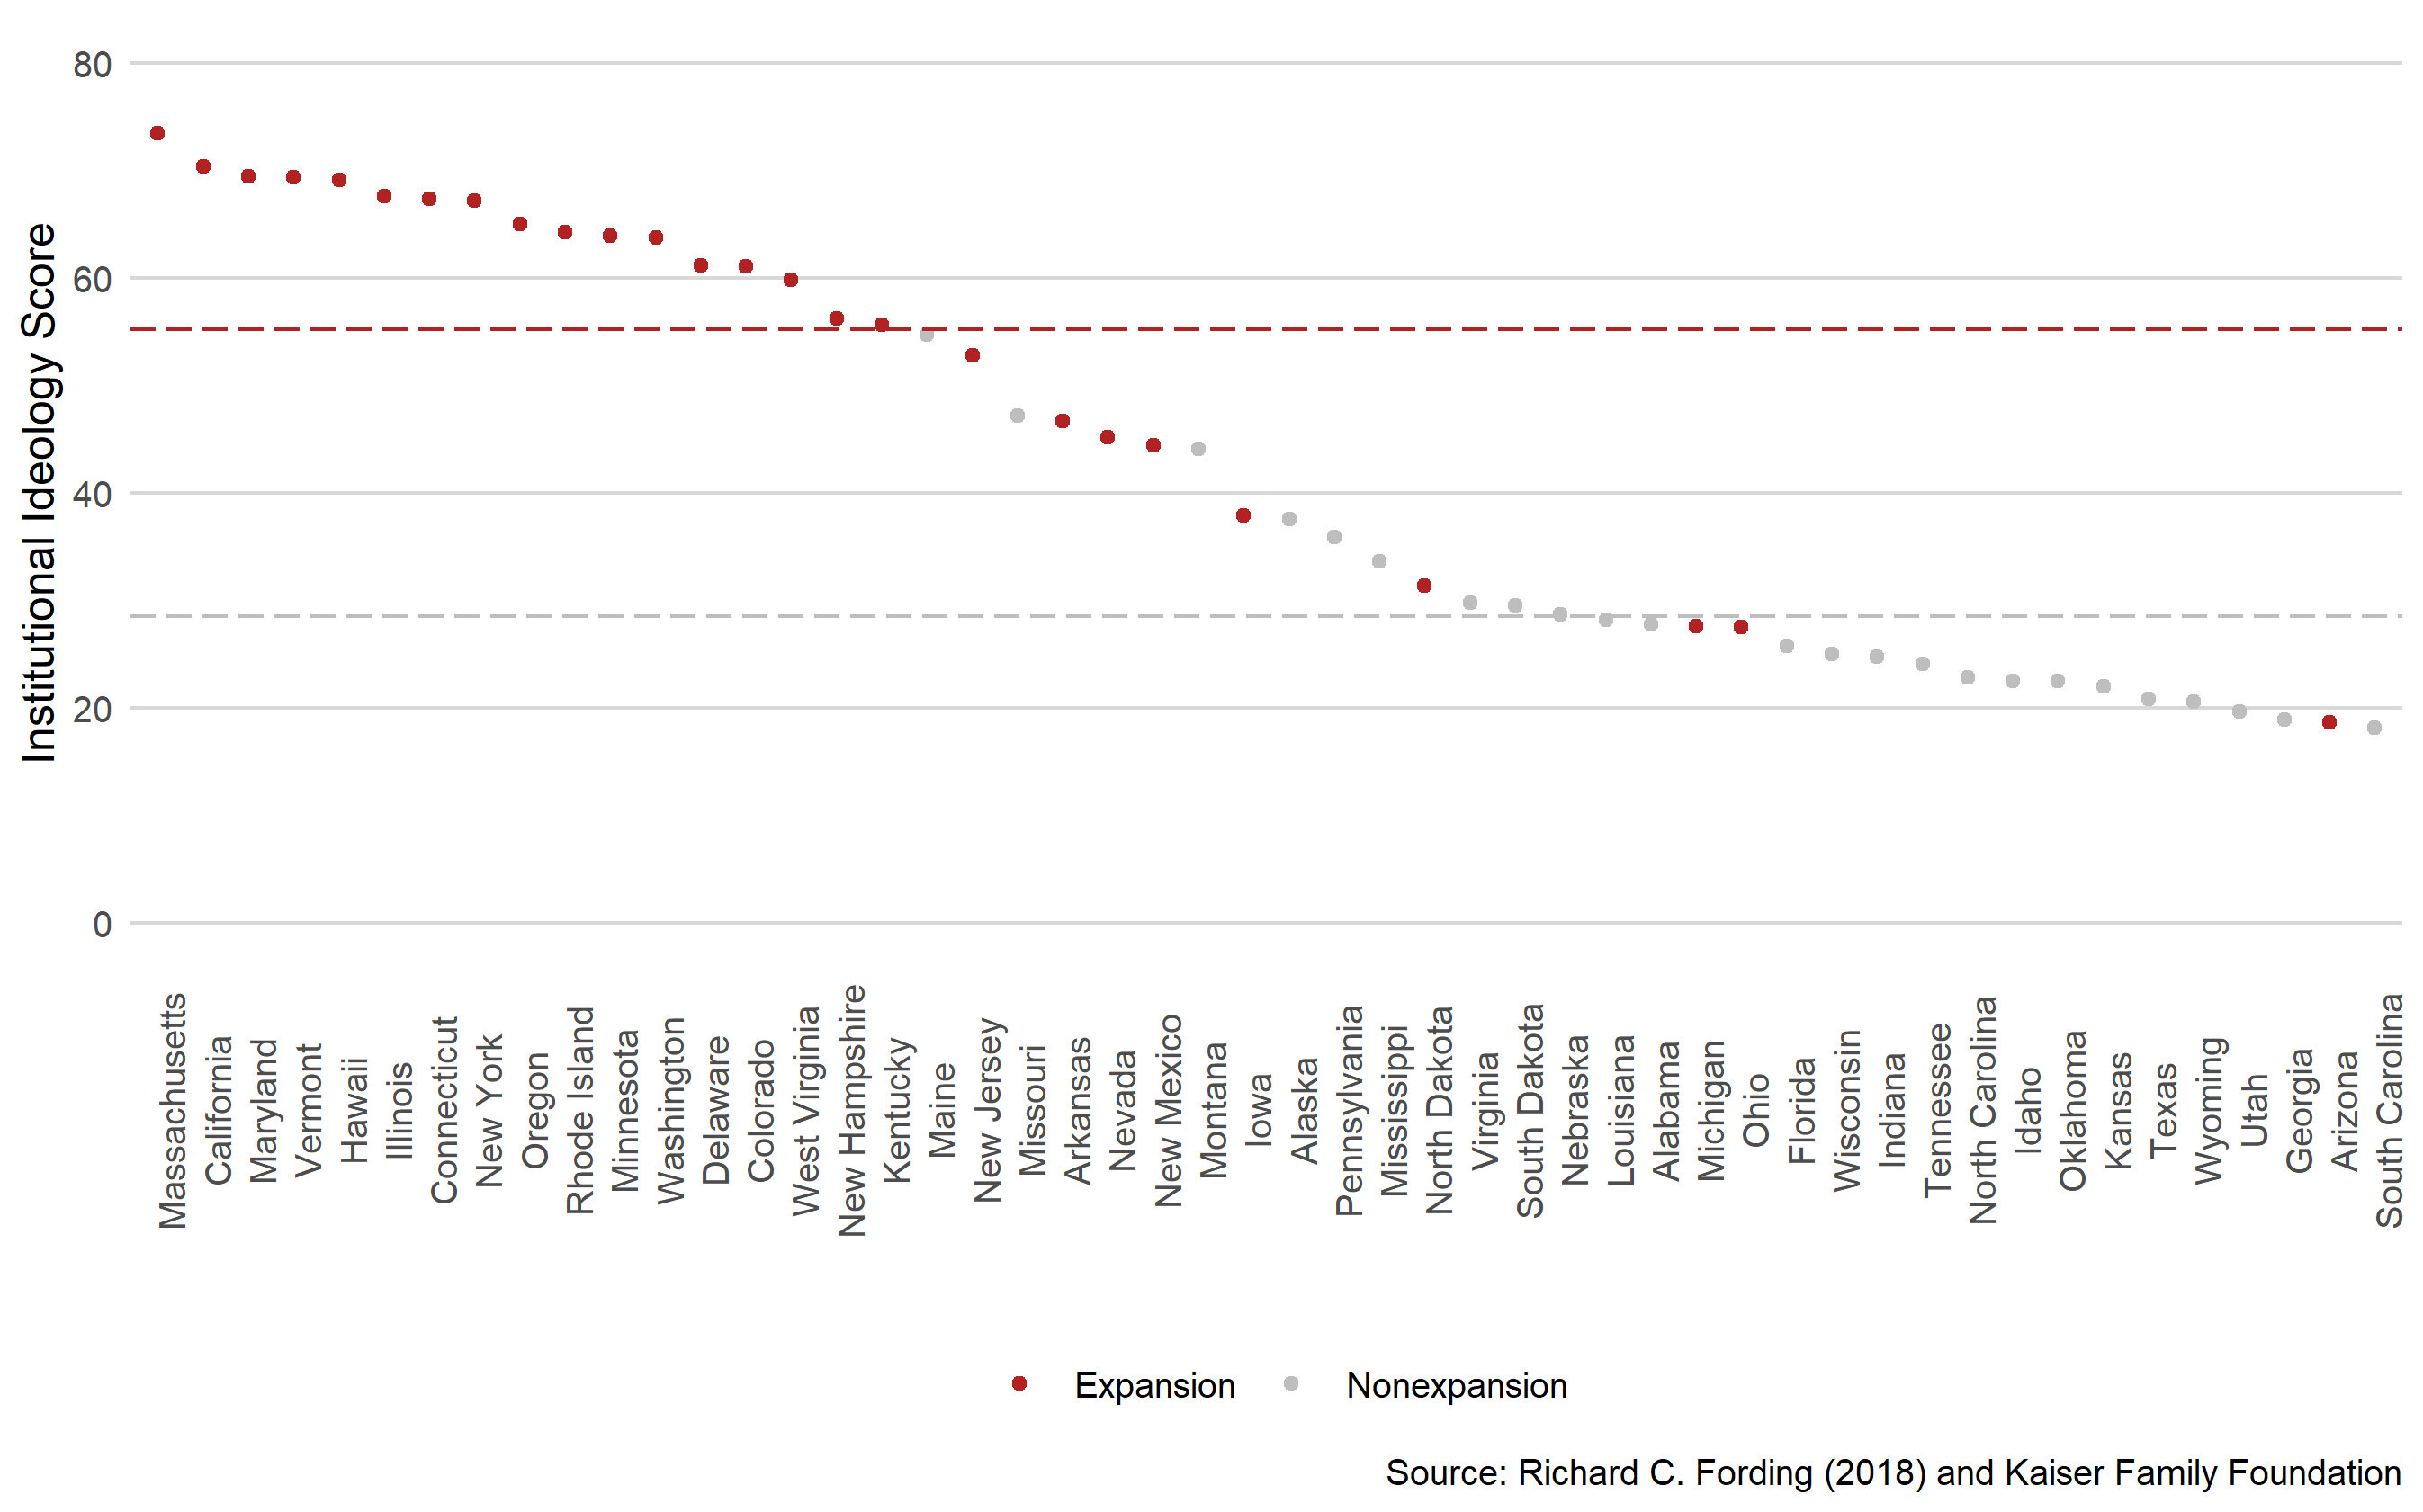
\includegraphics[scale=0.5]{01_Plots/political-expansion-plot.png}
    \end{center}
\end{frame}

\begin{frame}{Contributions: Substantive}
\begin{itemize}
    \item We estimate the treatment effect of 2014 Medicaid expansion on non-expansion states \bigskip
    
    \begin{itemize}
        \item We estimate -2 percentage point change, over 35 percent lower in absolute magnitude than ETT from Courtenmanche et al. (2017) \bigskip 
    \end{itemize}

    \item We examine how factors associated with Republican governance might drive this difference \bigskip
    
    \begin{itemize}
        \item We find a consistent positive association between Republican governance and our predicted uninsurance rates under treatment \bigskip 
    \end{itemize}
    \end{itemize}
\end{frame}

\begin{frame}{Contributions: Methodological}
\begin{itemize}
    \item We outline the assumptions necessary to estimate a ``synthetic treatment'' using longitudinal data \bigskip
    
    \item We generate balancing weights that account for hierarchical data structure (reduce the variance) \bigskip
    
    \item Our balancing weights account for measurement error in our covariates (reduce the bias) \bigskip
    \end{itemize}
\end{frame}

\section{Identification}

\subsection{Target estimand}

\begin{frame}{Target estimand}

$$
N_c^{-1}\sum_{s: A_s = 0} \sum_{c = 1}^{n_s} (Y_{scT}^1 - Y_{scT}^0)
$$

\begin{itemize}
    \item $Y$ is the uninsurance rate (``county'' level) \bigskip
    \item $A$ is the decision to expand Medicaid (state level) \bigskip
    \item $T$ is the post-treatment time period (2014)
\end{itemize}
\end{frame}

\subsection{Identification}

\begin{frame}{Identifying Assumptions}

\begin{itemize}
    \item SUTVA \bigskip
    \begin{itemize}
        \item No spillovers; only one version of treatment \bigskip
    \end{itemize}
    \item No anticipatory treatment effects \bigskip
    \begin{itemize}
        \item For $t < T$, $Y_{sct}^0 = Y_{sct}$ \bigskip
    \end{itemize}
\end{itemize}

\end{frame}

\begin{frame}{Treatment assignment}
    \begin{center}
	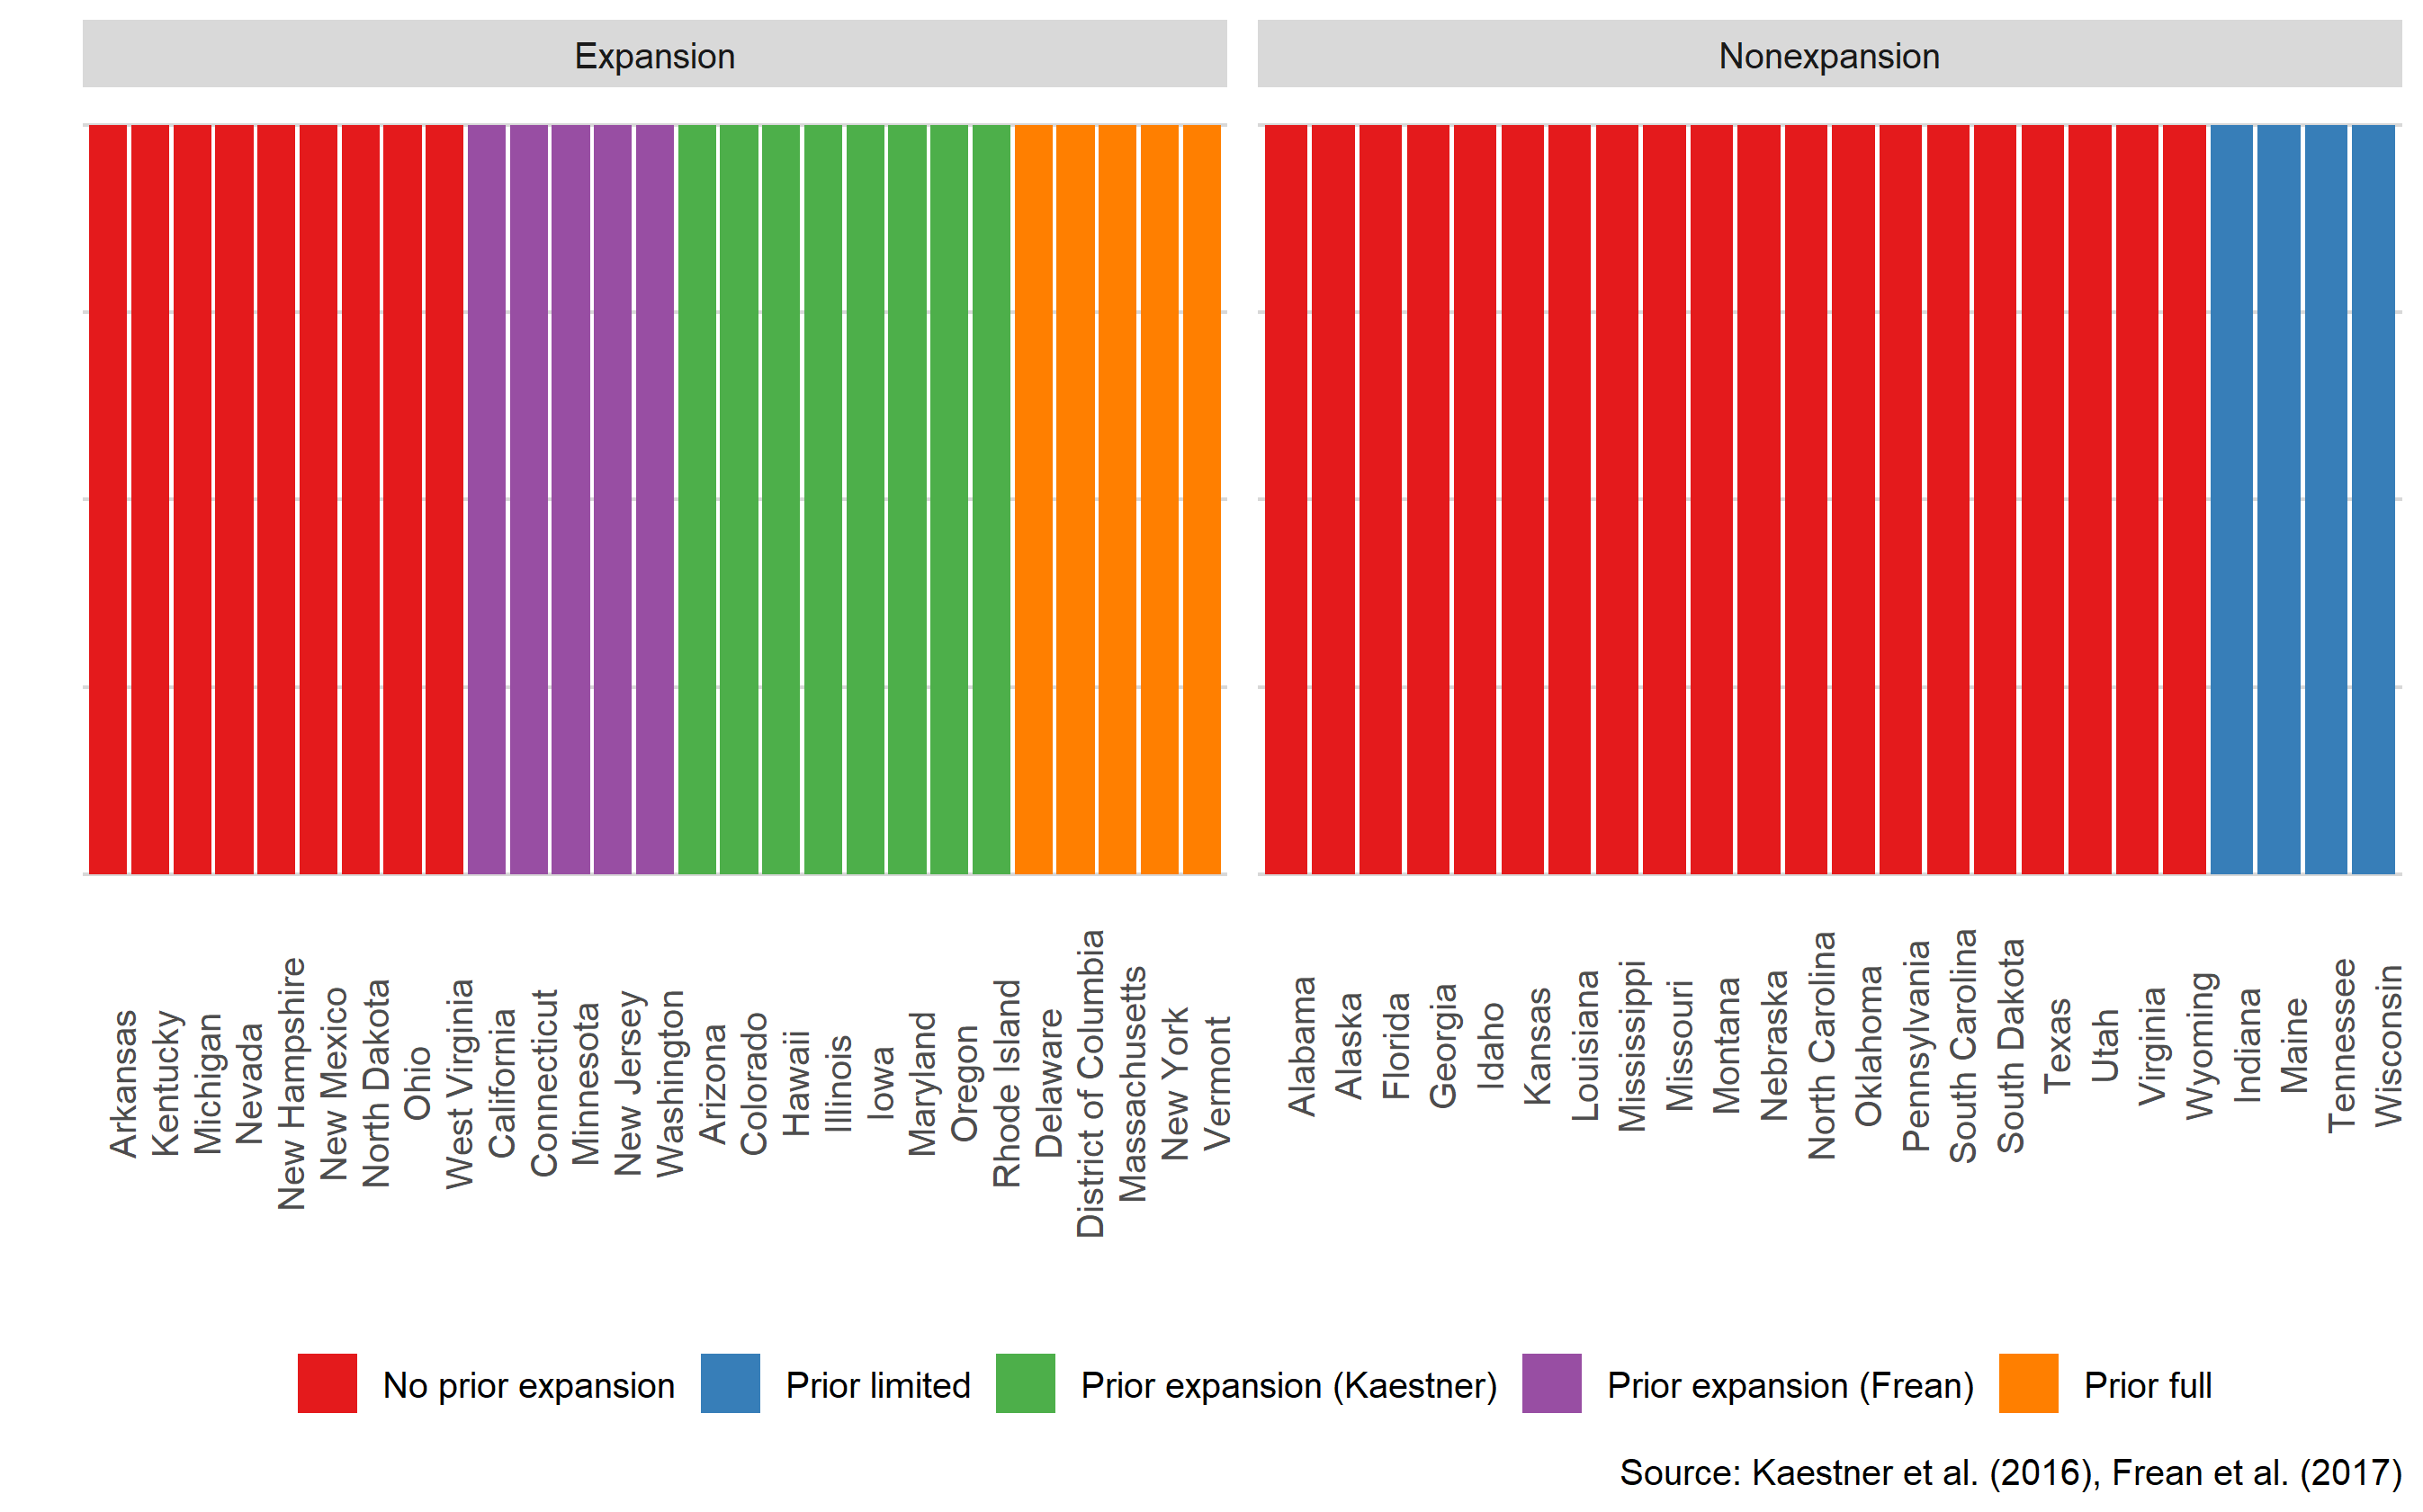
\includegraphics[scale=0.5]{01_Plots/expansion-heterogeneity.png}
    \end{center}
\end{frame}

\begin{frame}{Treatment assignment}
    \begin{center}
	
\includegraphics[scale=0.5]{01_Plots/expansion-heterogeneity-classification.png}  
    \end{center}
\end{frame}

\begin{frame}{Identifying Assumptions}
    \item Positivity \bigskip
    \begin{itemize}
        \item $1 > \pi(X_{sn_1}, ..., X_{sn_s}) > 0$ \bigskip
    \end{itemize}
    \item No unmeasured confounding \bigskip
    \begin{itemize}
        \item $Y^a_{sc} \perp A_s | X_{sc}$ \bigskip 
    \end{itemize}
\end{frame}

\begin{frame}{Covariates}
\begin{itemize}
    \item Uninsurance rates (2011-13) \bigskip
    \item Unemployment rates (2011-13) \bigskip
    \item ``Time-invariant'' demographics (2011-13 averages) \bigskip
    \begin{itemize}
        \item Age, sex, race, ethnicity, disability, foreign born, citizenship, education, income-to-poverty ratio, urban residence, married, children \bigskip
    \end{itemize}
    \item Political partisan composition \bigskip
    \begin{itemize}
        \item Republican governor, Republican lower chamber control, Republican total control
    \end{itemize}
\end{itemize}
\end{frame}

\begin{frame}{Data Source}
    \begin{itemize}
    \item American Community Survey (ACS) microdata from 2011-2014 \bigskip 
    \item Approximately three million individuals surveyed annually from across the United States \bigskip 
    \item Each individual has an associated survey weight and 80 sets of replicate survey weights \bigskip 
    \item Aggregate data to consistent public use microdata area (CPUMA) level
    \end{itemize}
\end{frame}   

\begin{frame}{Problem: measurement error in covariates}
    \begin{itemize}
        \item All ACS generated covariates are estimates \bigskip
        \begin{itemize}
            \item We observe $W_{sc}$, but we need $X_{sc}$ \bigskip
            \item $Y_{sc}^a \perp A_{sc} \mid X_{sc} \centernot\implies Y_{sc}^a \perp A_{sc} \mid W_{sc}$ \bigskip
        \end{itemize}
        \item $W_{sc} = X_{sc} + v_{sc}$, where $v_{sc} \sim N(0, \Sigma_{vv, sc})$ \bigskip
        \item Sample sizes range from [X, Z] \bigskip
    \end{itemize}
\end{frame}

\begin{frame}{Parametric assumptions}
    \begin{itemize}
        \item Linearity of outcome model \bigskip
        \begin{itemize}
            \item $Y_{sc} = \alpha + X_{sc}^T\beta + \epsilon_{sc} + \nu_s$ \bigskip
        \end{itemize}
        \item Linearity of $X_{cs}$ in $W_{cs}$ \bigskip 
        \begin{itemize}
            \item $\mathbb{E}\{X_{sc} \mid W_{sc}, A_s = a\} = \eta_a(W_{sc}) = \mu_a + \kappa^T(W_{sc} - \mu_a)$ \bigskip
            \item $\kappa = (\Sigma_{XX} + \Sigma_{vv})^{-1}\Sigma_{XX}$ \bigskip
        \end{itemize}
        \item Potential outcome model \bigskip
        \begin{itemize}
            \item $Y_{sc}^1 = \alpha + \eta_1(W_{sc})^T\beta + (X_{sc} - \eta_1(W_{sc}))^T\beta + \epsilon_{sc} + \nu_{s}$
        \end{itemize}
    \end{itemize}
\end{frame}

\section{Estimation}

\begin{frame}{Overview}
    \begin{itemize}
        \item Balancing weights reweight covariate distribution of treated units to ``look like'' the covariate distribution of control units \bigskip
        \begin{itemize}
            \item Guard against specification searching \bigskip
            \item Limit extrapolation from the data \bigskip
            \item Makes our comparisons explicit \bigskip
        \end{itemize}
        \item Existing methods often assume iid data, no measurement error in the covariates
    \end{itemize}
\end{frame}

\begin{frame}{Balancing Weights}
    \begin{itemize}
        \item We generate weights that satisfy the following constraints:
    \end{itemize}
    
    $$
    \mathcal{W}:= \{w: (\sum_{s,c: A_s = 1}\gamma_{sc}\hat{\eta}_1(W_{sc}) - \bar{W}_0) \le \delta, w_i > 0, w^T1 = N_1\}
    $$
    
    \begin{itemize}
        \item We estimate $\hat{\eta}_a(W_{sc})$ using replicate survey weights on the ACS microdata files \bigskip
        \begin{itemize}
            \item ``Regression-calibratation'' methods are a much-studied topic (``the poor man's imputation'' -- Raymond Carroll) \bigskip
        \end{itemize}
        \item $\bar{W}_0$ is an estimate of the (population-weighted) mean covariate values for the control-units
    \end{itemize}
\end{frame}

\begin{frame}{How to choose $\delta$?}
    \begin{itemize}
        \item Typically $\delta > 0$ because we have a lack of covariate overlap in the observed data \bigskip
        \item To minimize this bias, we must choose $\delta$ using prior knowledge about what covariates are likely to be most predictive of treatment response \bigskip
        \item In contrast to the synthetic controls literature, we cannot in general use prior values of the outcome to learn the optimal $\delta$ \bigskip
    \end{itemize}
\end{frame}

\begin{frame}{Balancing Weights}
    \begin{itemize}
        \item For fixed $\delta$, our goal is to minimize the variance of our estimator \bigskip
        \item Assume that $Var(\epsilon_{sc})$ and $Var(v_s)$ are constant across units \bigskip
        $$
        \arg\min_{w \in \mathcal{W}}\sum_{s: A_s = 1}(\sum_{c = 1}^{n_s}w_{sc}^2 + \sum_{c \ne d}\rho w_{sc}w_{sd})
        $$
        \item This is a modification of the Stable Balancing Weights objective (Zubizaretta (2015))
    \end{itemize}
\end{frame}

\begin{frame}{What if $\delta$ are large?}
    \begin{itemize}
        \item Extrapolation using ridge-regression augmented weights (\cite{ben2018augmented}) \bigskip
    \end{itemize}
    
    $$
    \gamma^{sbw} + (\hat{\eta}_1(W_1)^T\gamma^{sbw} - \bar{W}_0)^T(\hat{\eta}_1(W_1)^T\hat{\eta}_1(W_1) + \lambda I_d)^{-1}\hat{\eta}_1(W_1)^T
    $$
    \bigskip
    \begin{itemize}
        \item Changing the target estimand: overlap average treatment effect (\cite{li2018balancing})
    \end{itemize}
\end{frame}

\begin{frame}{Inference}
    \begin{itemize}
        \item Preferred estimates use the leave-one-state-out jackknife, conditional on our adjustment $\hat{\eta}_a(W_{ij})$ \bigskip
        \item We also create confidence intervals the leave-one-state-out jackknife recalculating $\hat{\eta}_a$ each time \bigskip
        \item More precise inference in this setting is a problem beyond the scope of this paper
    \end{itemize}
\end{frame}

\section{Results}

\subsection{Question One}

\begin{frame}{Question One}
    \begin{itemize}
        \item What is our estimate of $\psi$? \bigskip
        \begin{itemize}
            \item Is it robust to different sets of weights $\gamma$? \bigskip
            \begin{itemize}
                \item Extrapolation versus imbalances \bigskip
            \end{itemize}
            \item Is it robust to excluding ``early expansion'' states? \bigskip
            \item Is it robust to alternate specifications of $\eta(W_{sc})$? \bigskip
        \end{itemize}
    \end{itemize}
\end{frame}

\begin{frame}{Covariate Balance: Primary Dataset}
    \begin{center}
	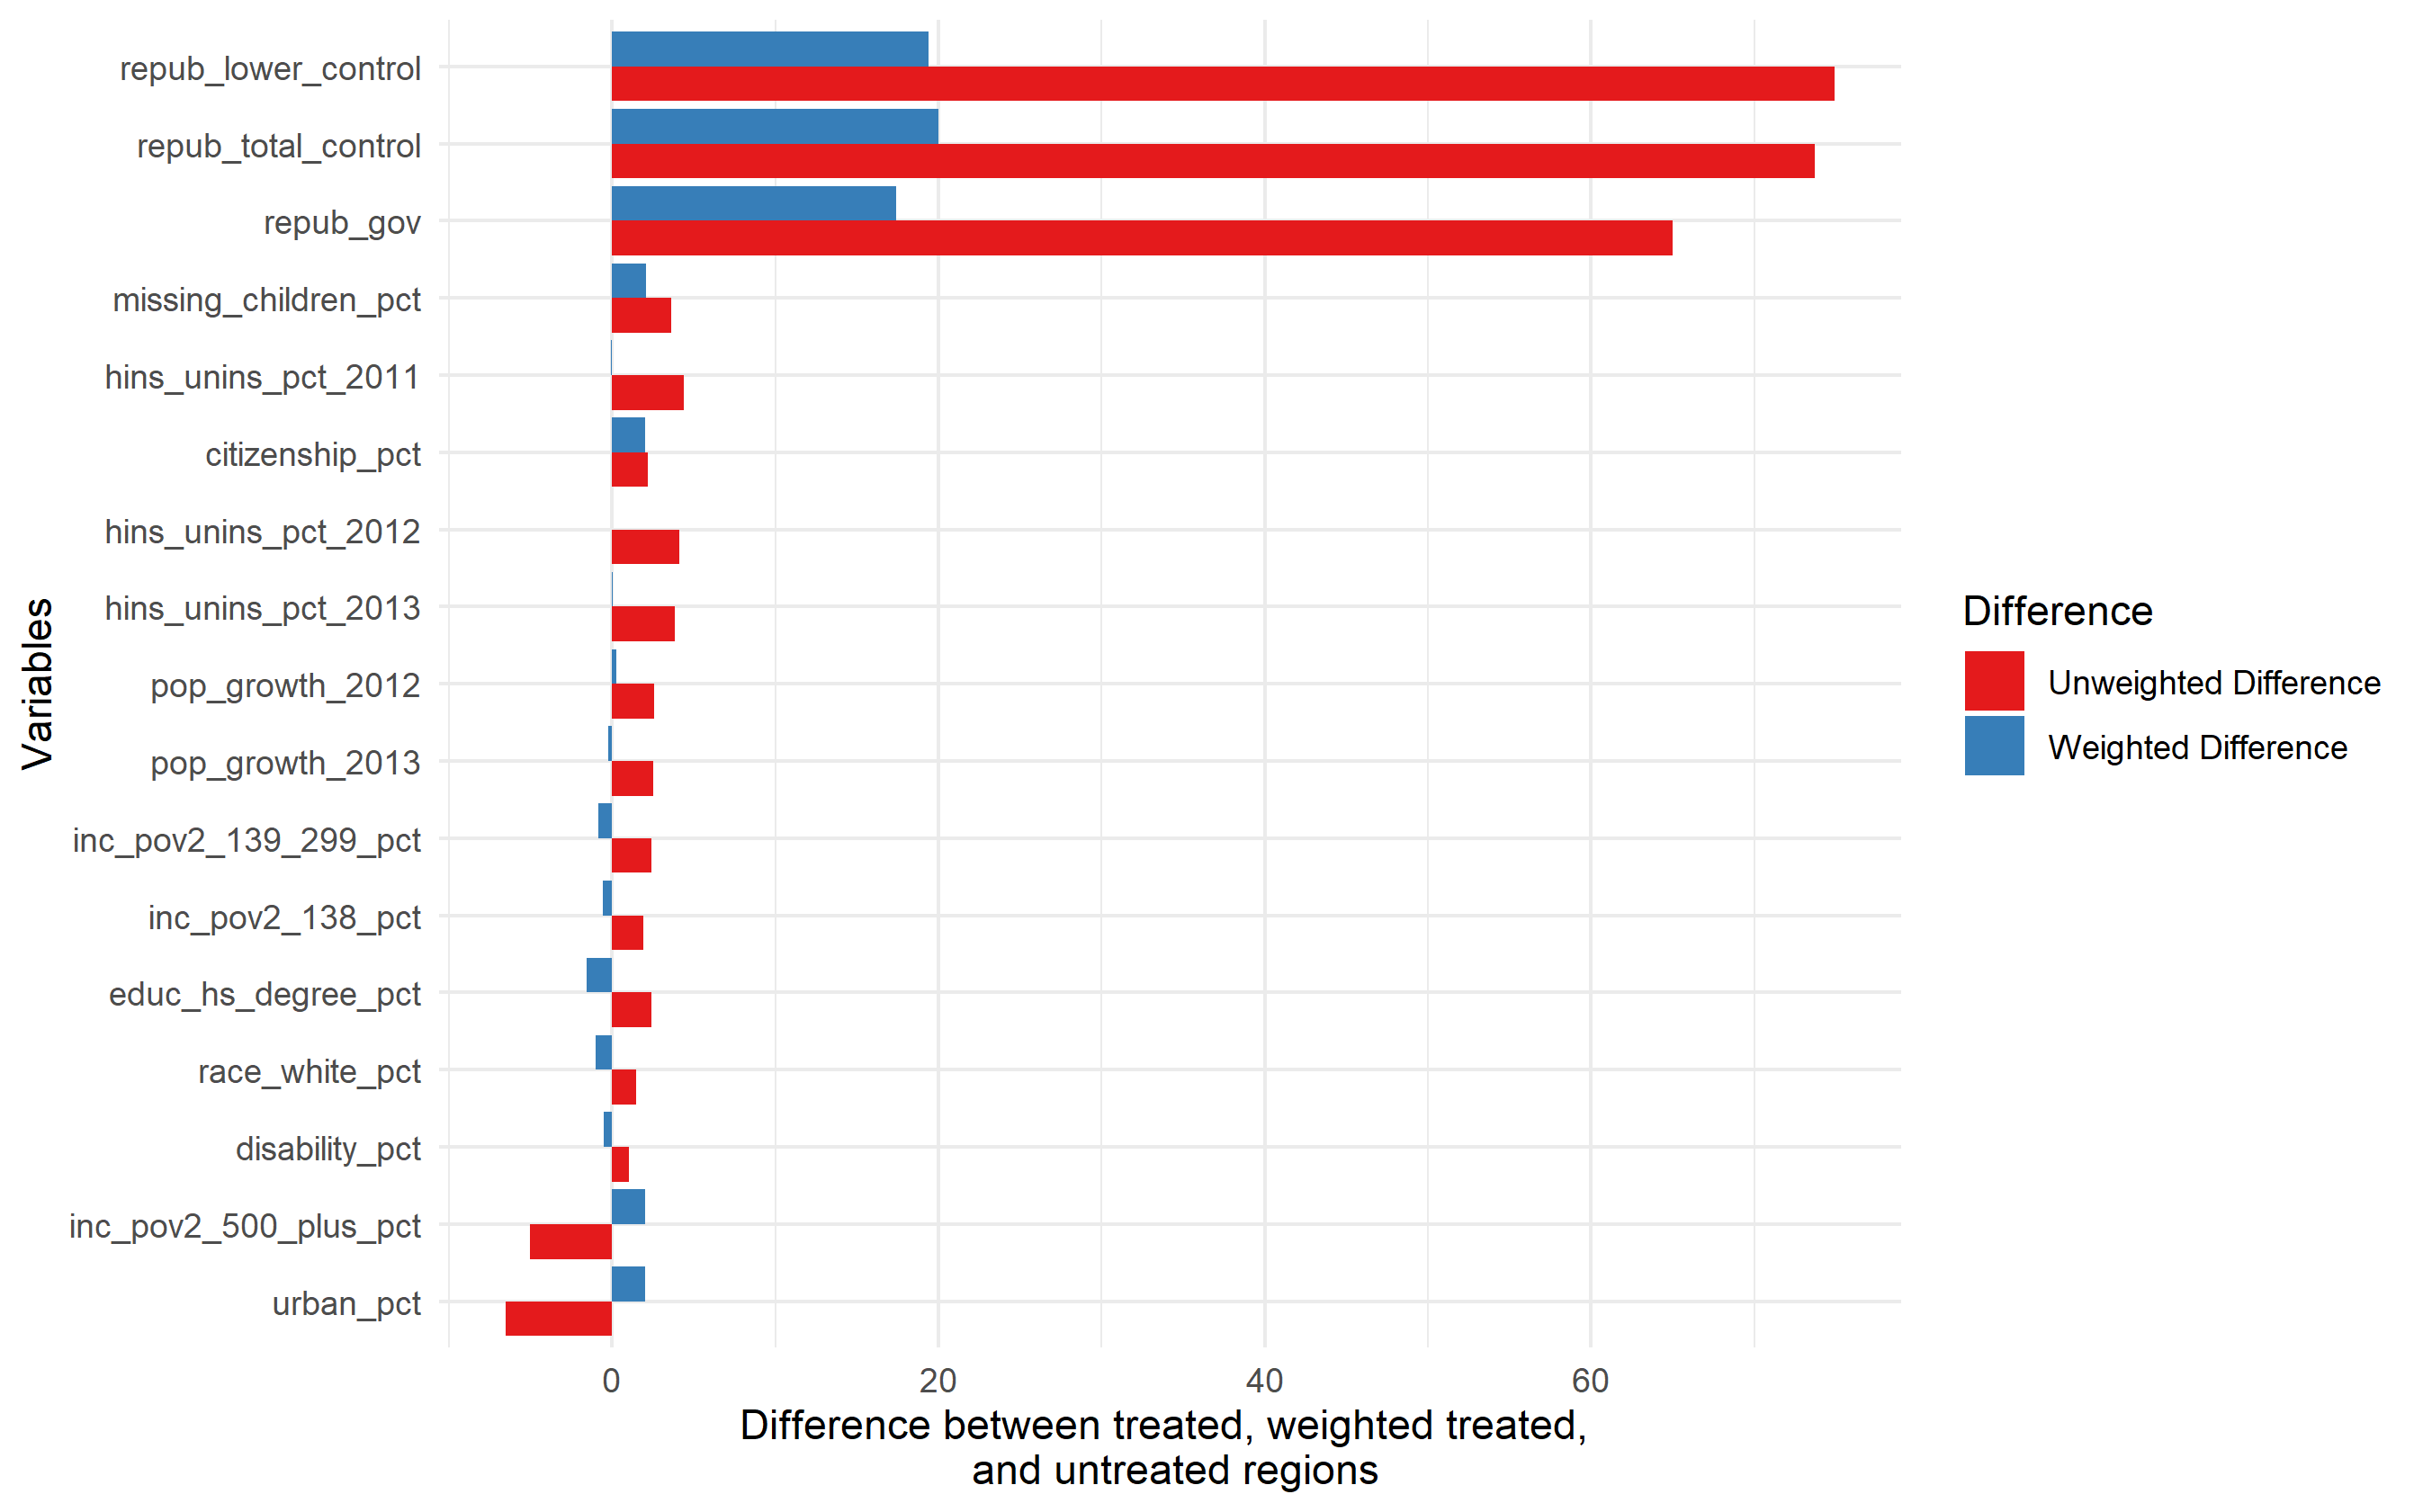
\includegraphics[scale=0.5]{01_Plots/balance-plot-etuc1.png}
    \end{center}
\end{frame}

\begin{frame}{Primary Point Estimates}

\begin{table}[ht]
\begin{tabular}{llrll}
  \toprule
Estimator & Estimate & 95 percent CI (lower, upper)\\ 
  \midrule
  H-SBW & -2.00 & (-3.59, -0.40) \\ 
  BC-HSBW & -2.14 & (-3.57, -0.71) \\ 
  SBW & -1.81 & (-3.60, -0.02) \\ 
  BC-SBW & -1.89 & (-3.06, -0.73) \\ 
   \bottomrule
\end{tabular}
\caption{Primary point estimates and confidence intervals}
\label{tab:confintmain}
\end{table}
\end{frame}

\begin{frame}{Covariate Balance: Early Expansion Excluded}
    \begin{center}
	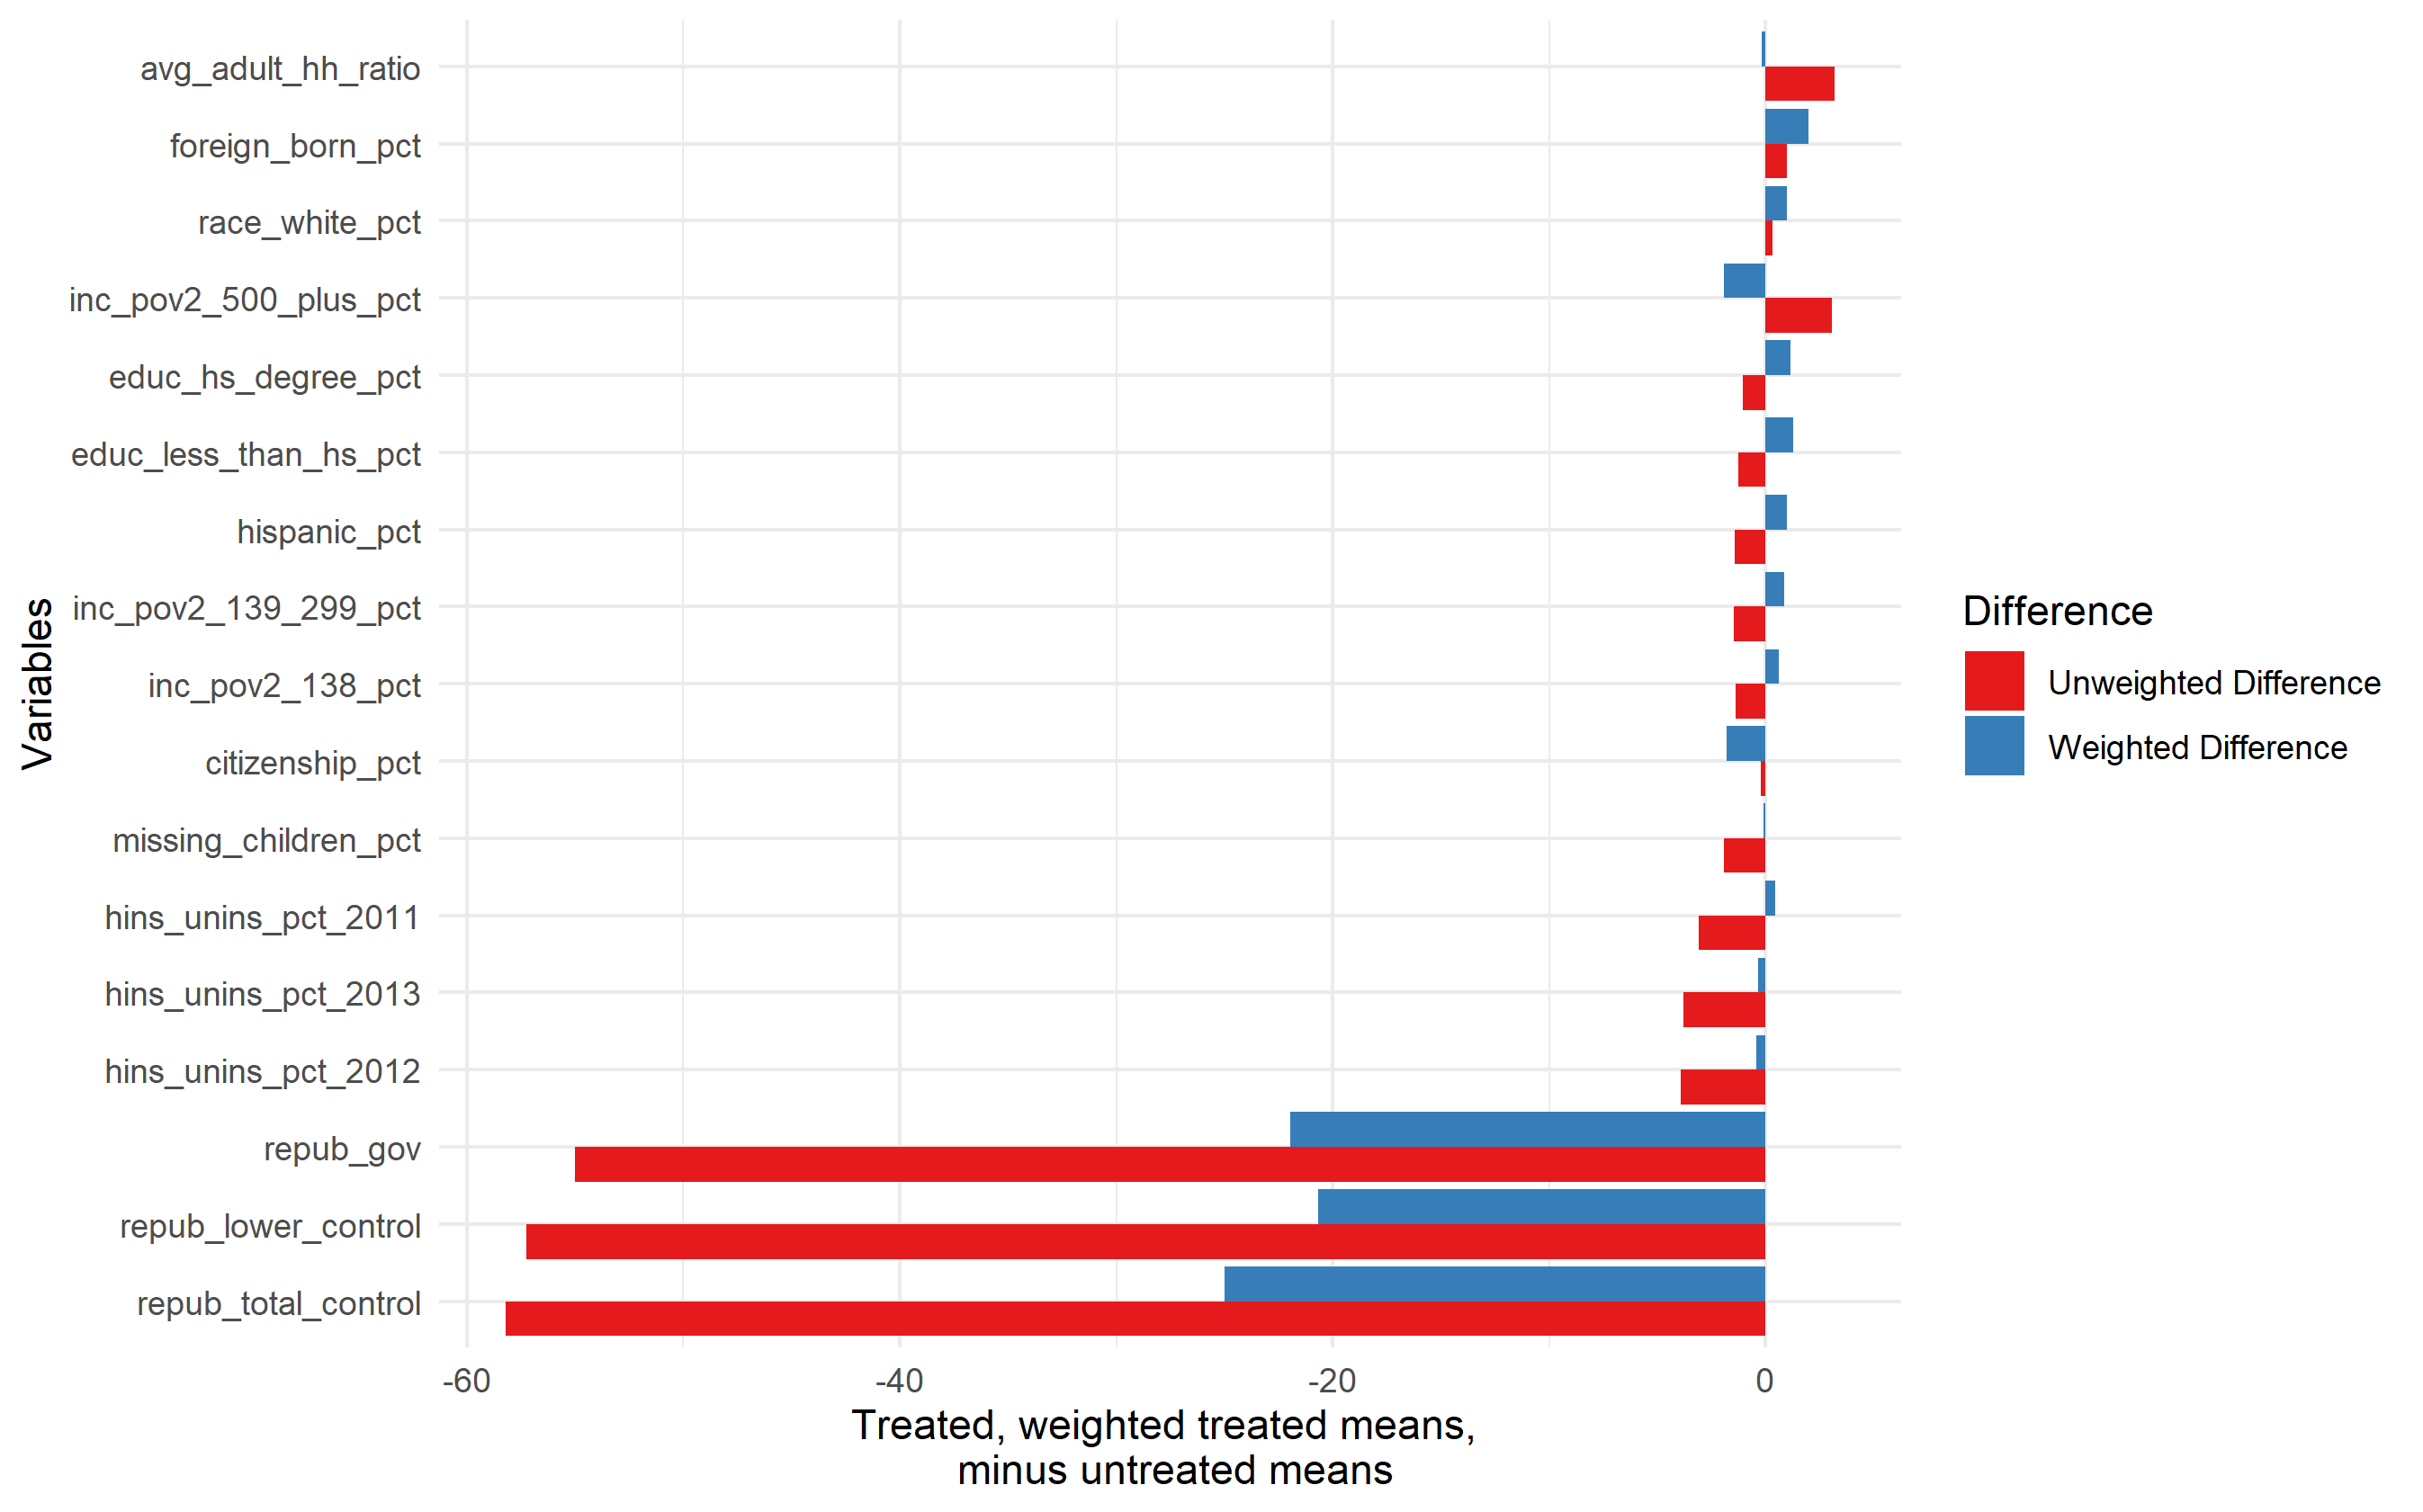
\includegraphics[scale=0.5]{01_Plots/balance-plot-etuc2.png}
    \end{center}
\end{frame}

\begin{frame}{Sensitivity analysis: no anticipatory treatment effects}
    \begin{table}[ht]
\centering
\begin{tabular}{llrll}
  \toprule
Weight type & Psihat & 95 Percent CI \\ 
  \midrule
H-SBW & -1.29 & (-2.45, -0.12) \\ 
BC-HSBW & -2.17 & (-3.65, -0.68) \\ 
SBW & -1.12 & (-2.23, -0.02) \\ 
BC-SBW & -1.93 & (-3.32, -0.54) \\ 
   \bottomrule
\end{tabular}
\caption{Early expansion excluded, point estimates}
\label{tab:confintmainc2}
\end{table}
\end{frame}

\begin{frame}{Robustness plot}

\begin{center}
	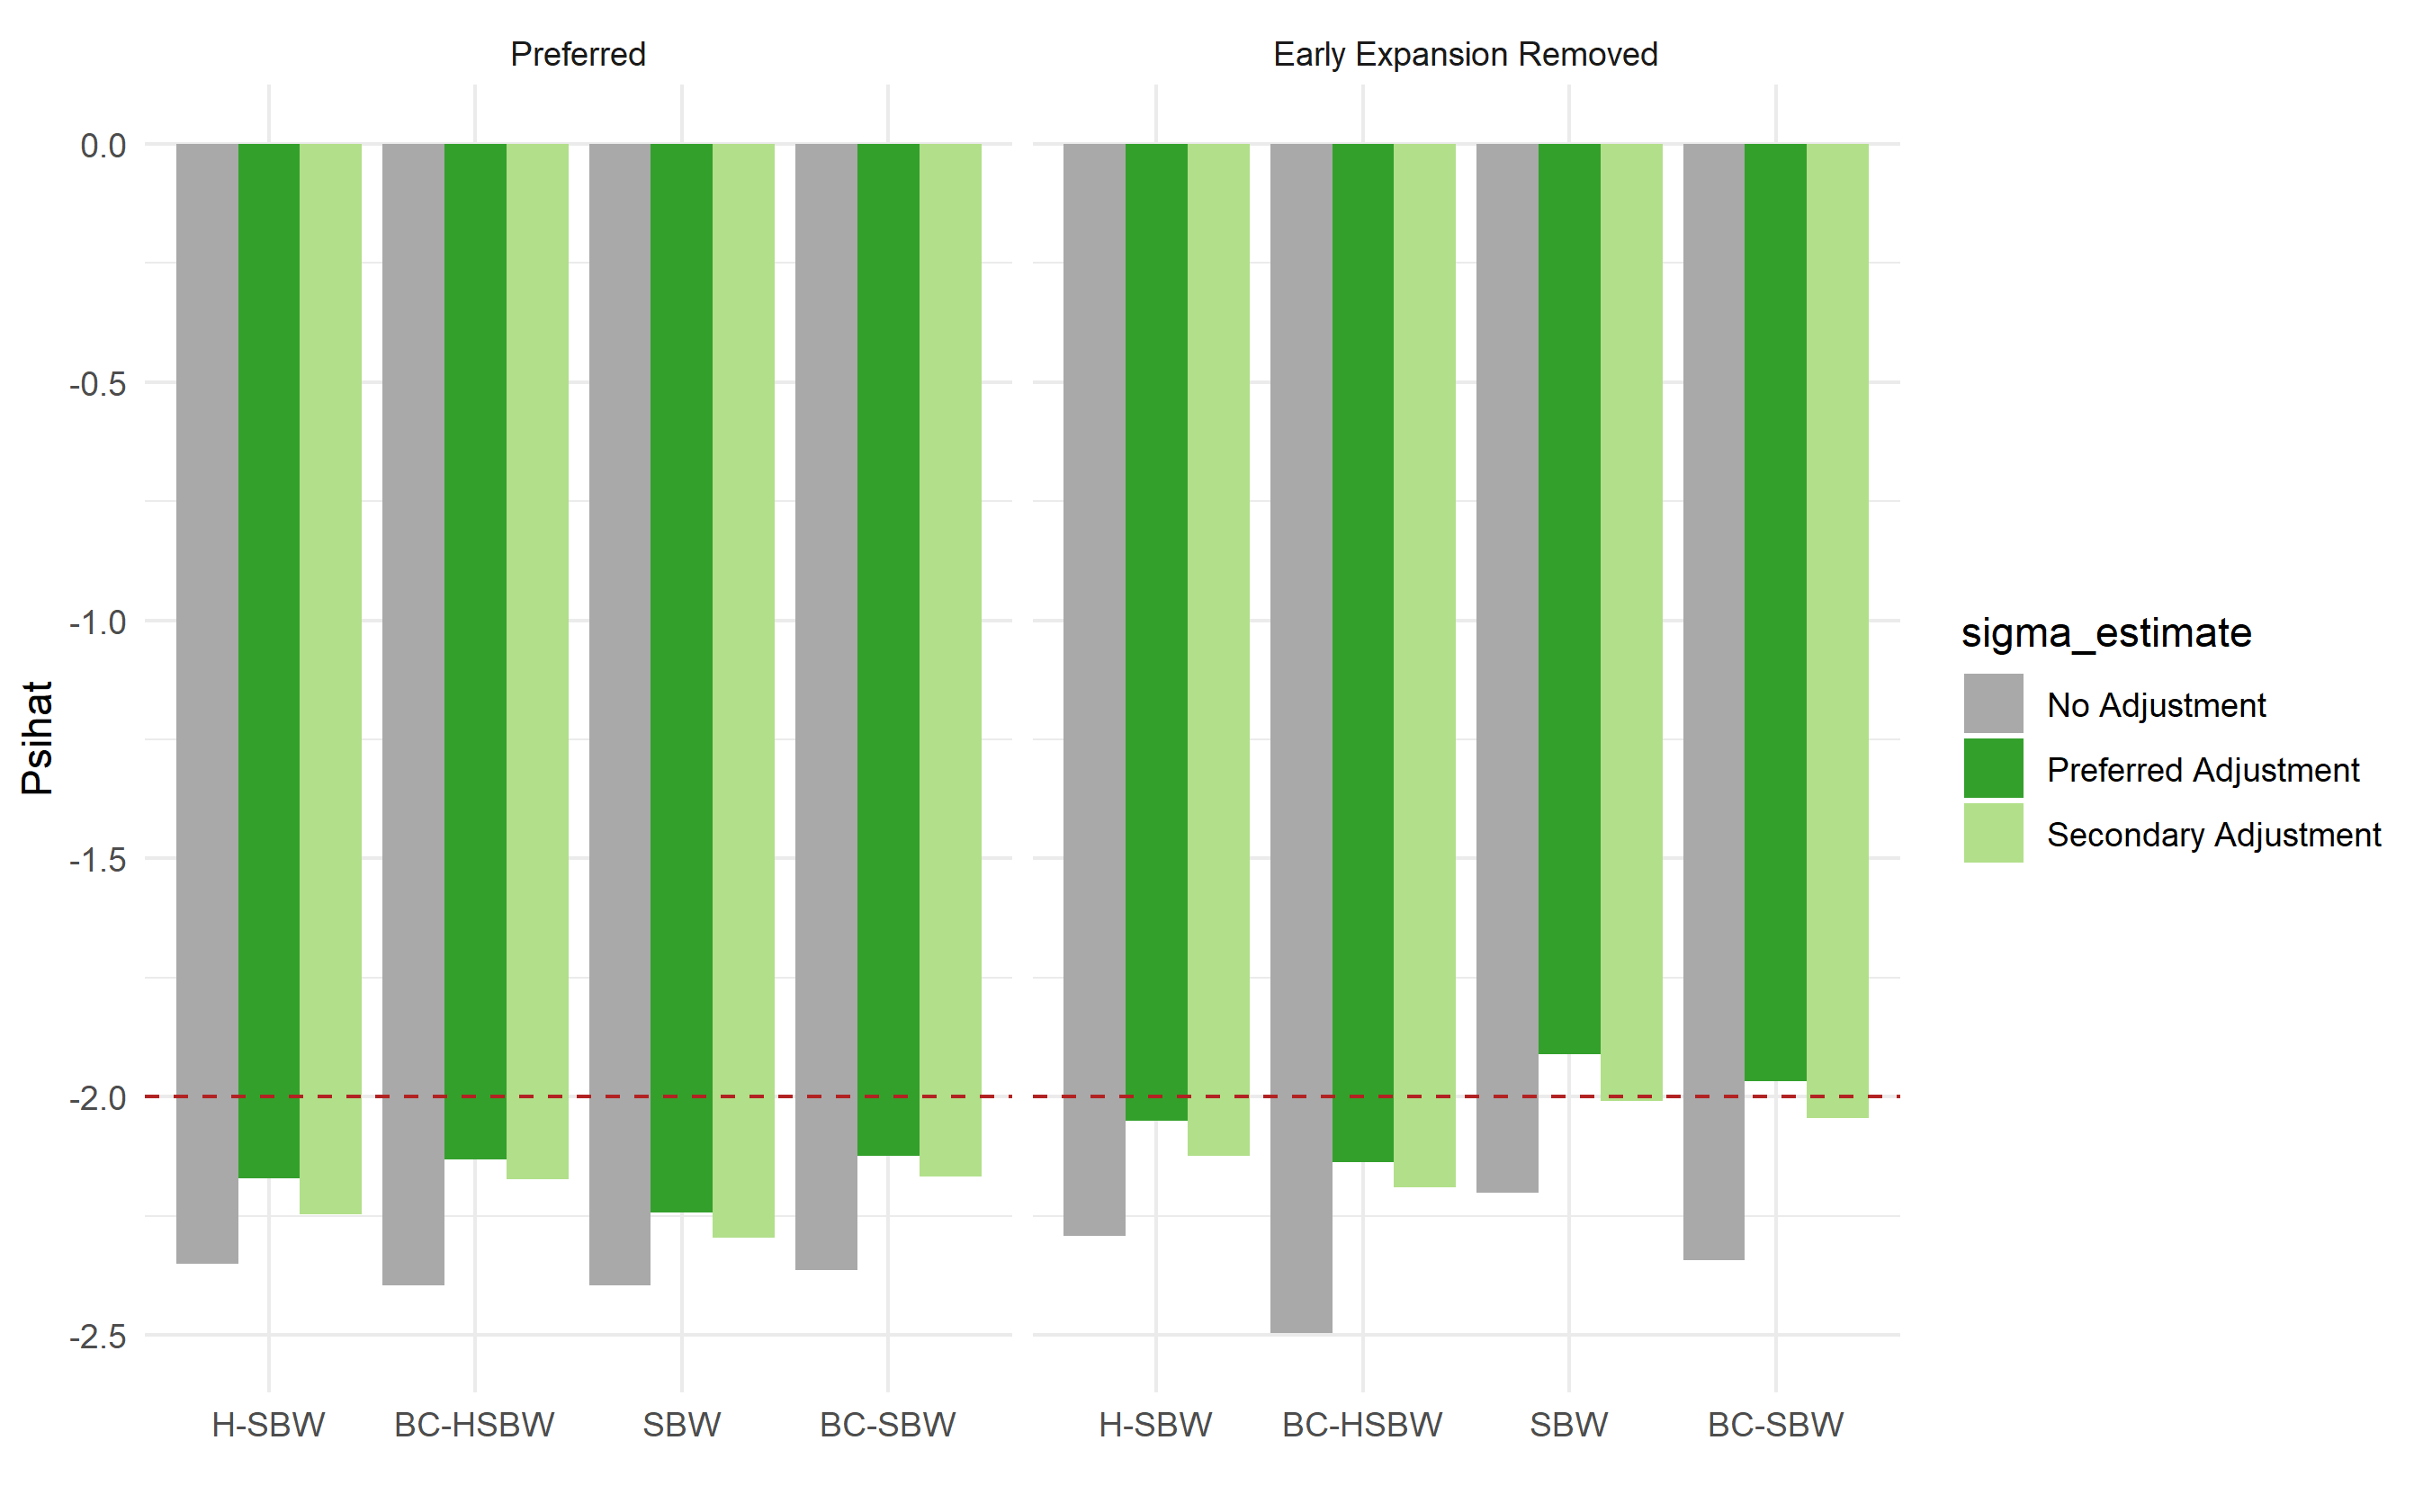
\includegraphics[scale=0.5]{01_Plots/all-estimates-c1c2.png}
\end{center}
\end{frame}

\subsection{Question Two}

\begin{frame}{Question Two}
    \begin{itemize}
        \item How sensitive is $\hat{\psi}$ to excluding different covariate sets $V$? \bigskip 
        \begin{itemize}
            \item Primarily interested in Republican governance indicators \bigskip
        \end{itemize}
        \item Let $\hat{\psi}_1$ be estimate excluding covariates, $\hat{\psi}_0$ be the original estimate using weights $\gamma_1$ and $\gamma_2$ \bigskip
        \item $\Delta = \hat{\psi}^1_1 - \hat{\psi}^1_0$ \bigskip
        \item $\mathbb{E}\{\Delta\} = (X_1^T\gamma_1 - X_1^T\gamma_0)^T\beta_X \approx (V_1^T\gamma_1 - V_1^T\gamma_0)^T\beta_V$
    \end{itemize}
\end{frame}

\begin{frame}{Heterogeneity across covariate groups}
\begin{center}
	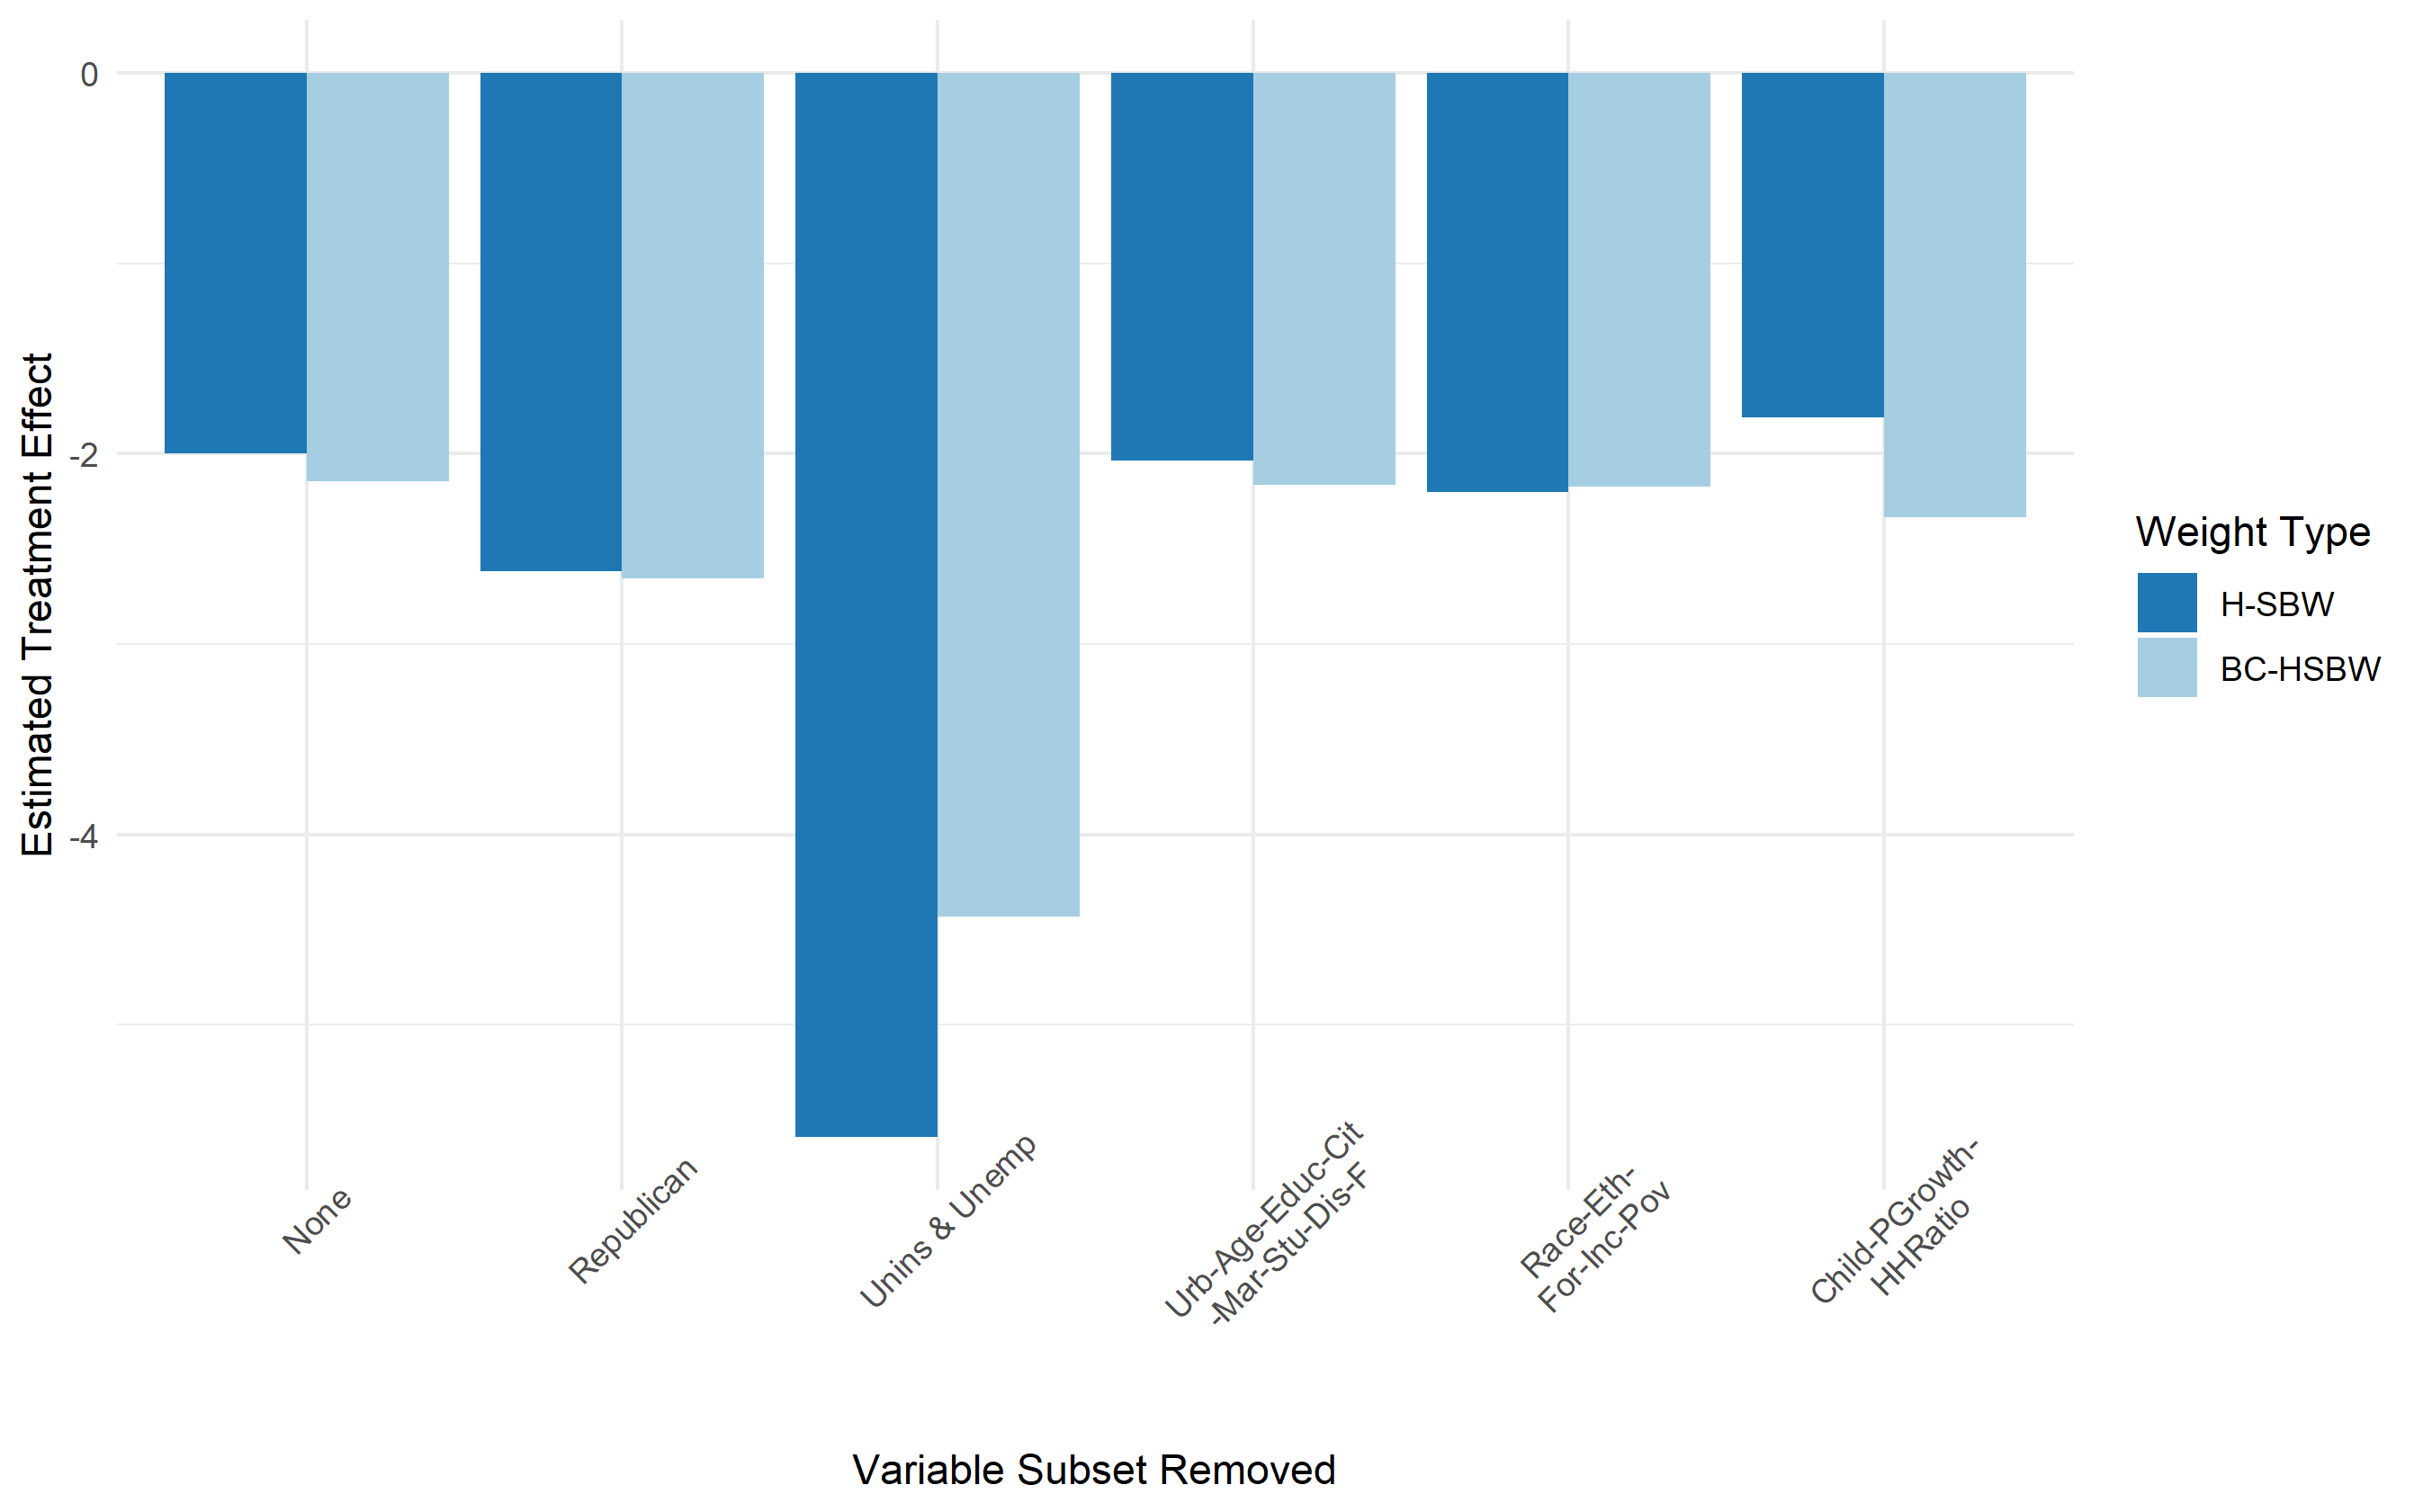
\includegraphics[scale=0.5]{01_Plots/loo-covariates-main-c1.png}
\end{center}
\end{frame}

\begin{frame}{Republican governance removal}
\begin{center}
	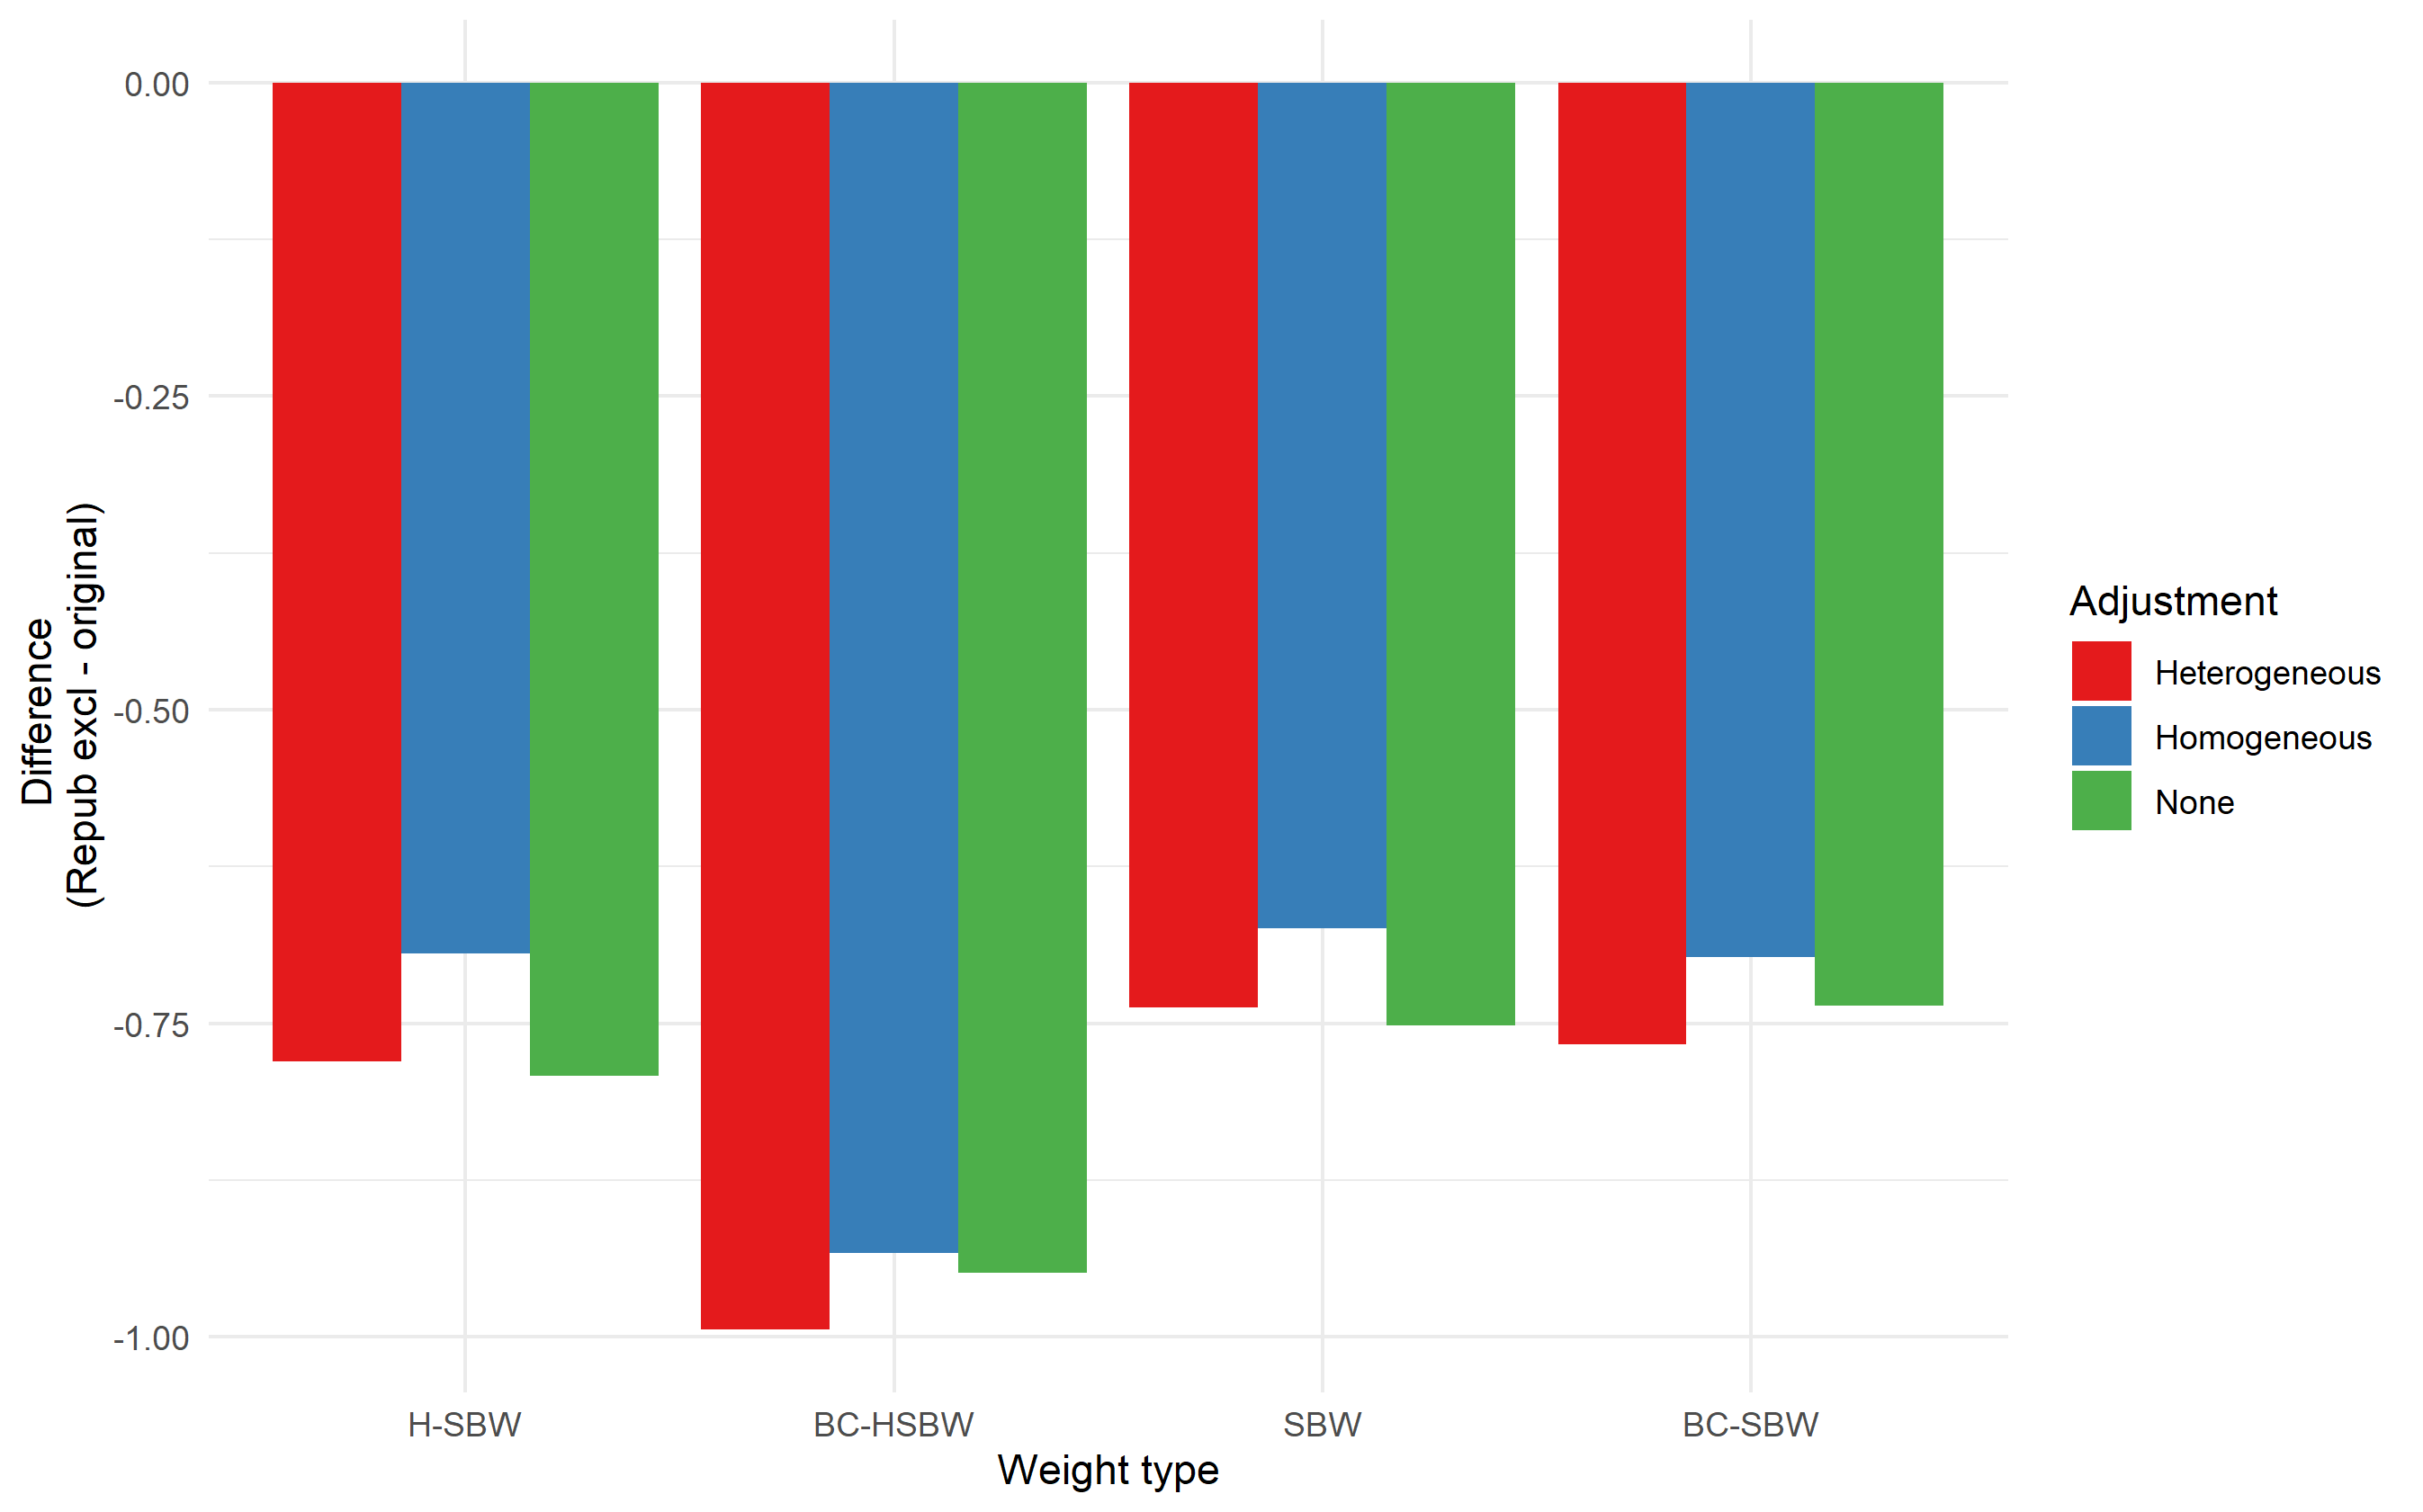
\includegraphics[scale=0.5]{01_Plots/repub-diff-c1-robustness.png}
\end{center}
\end{frame}

\begin{frame}{Sensitivity analysis: no anticipatory treatment effects}
    \begin{center}
	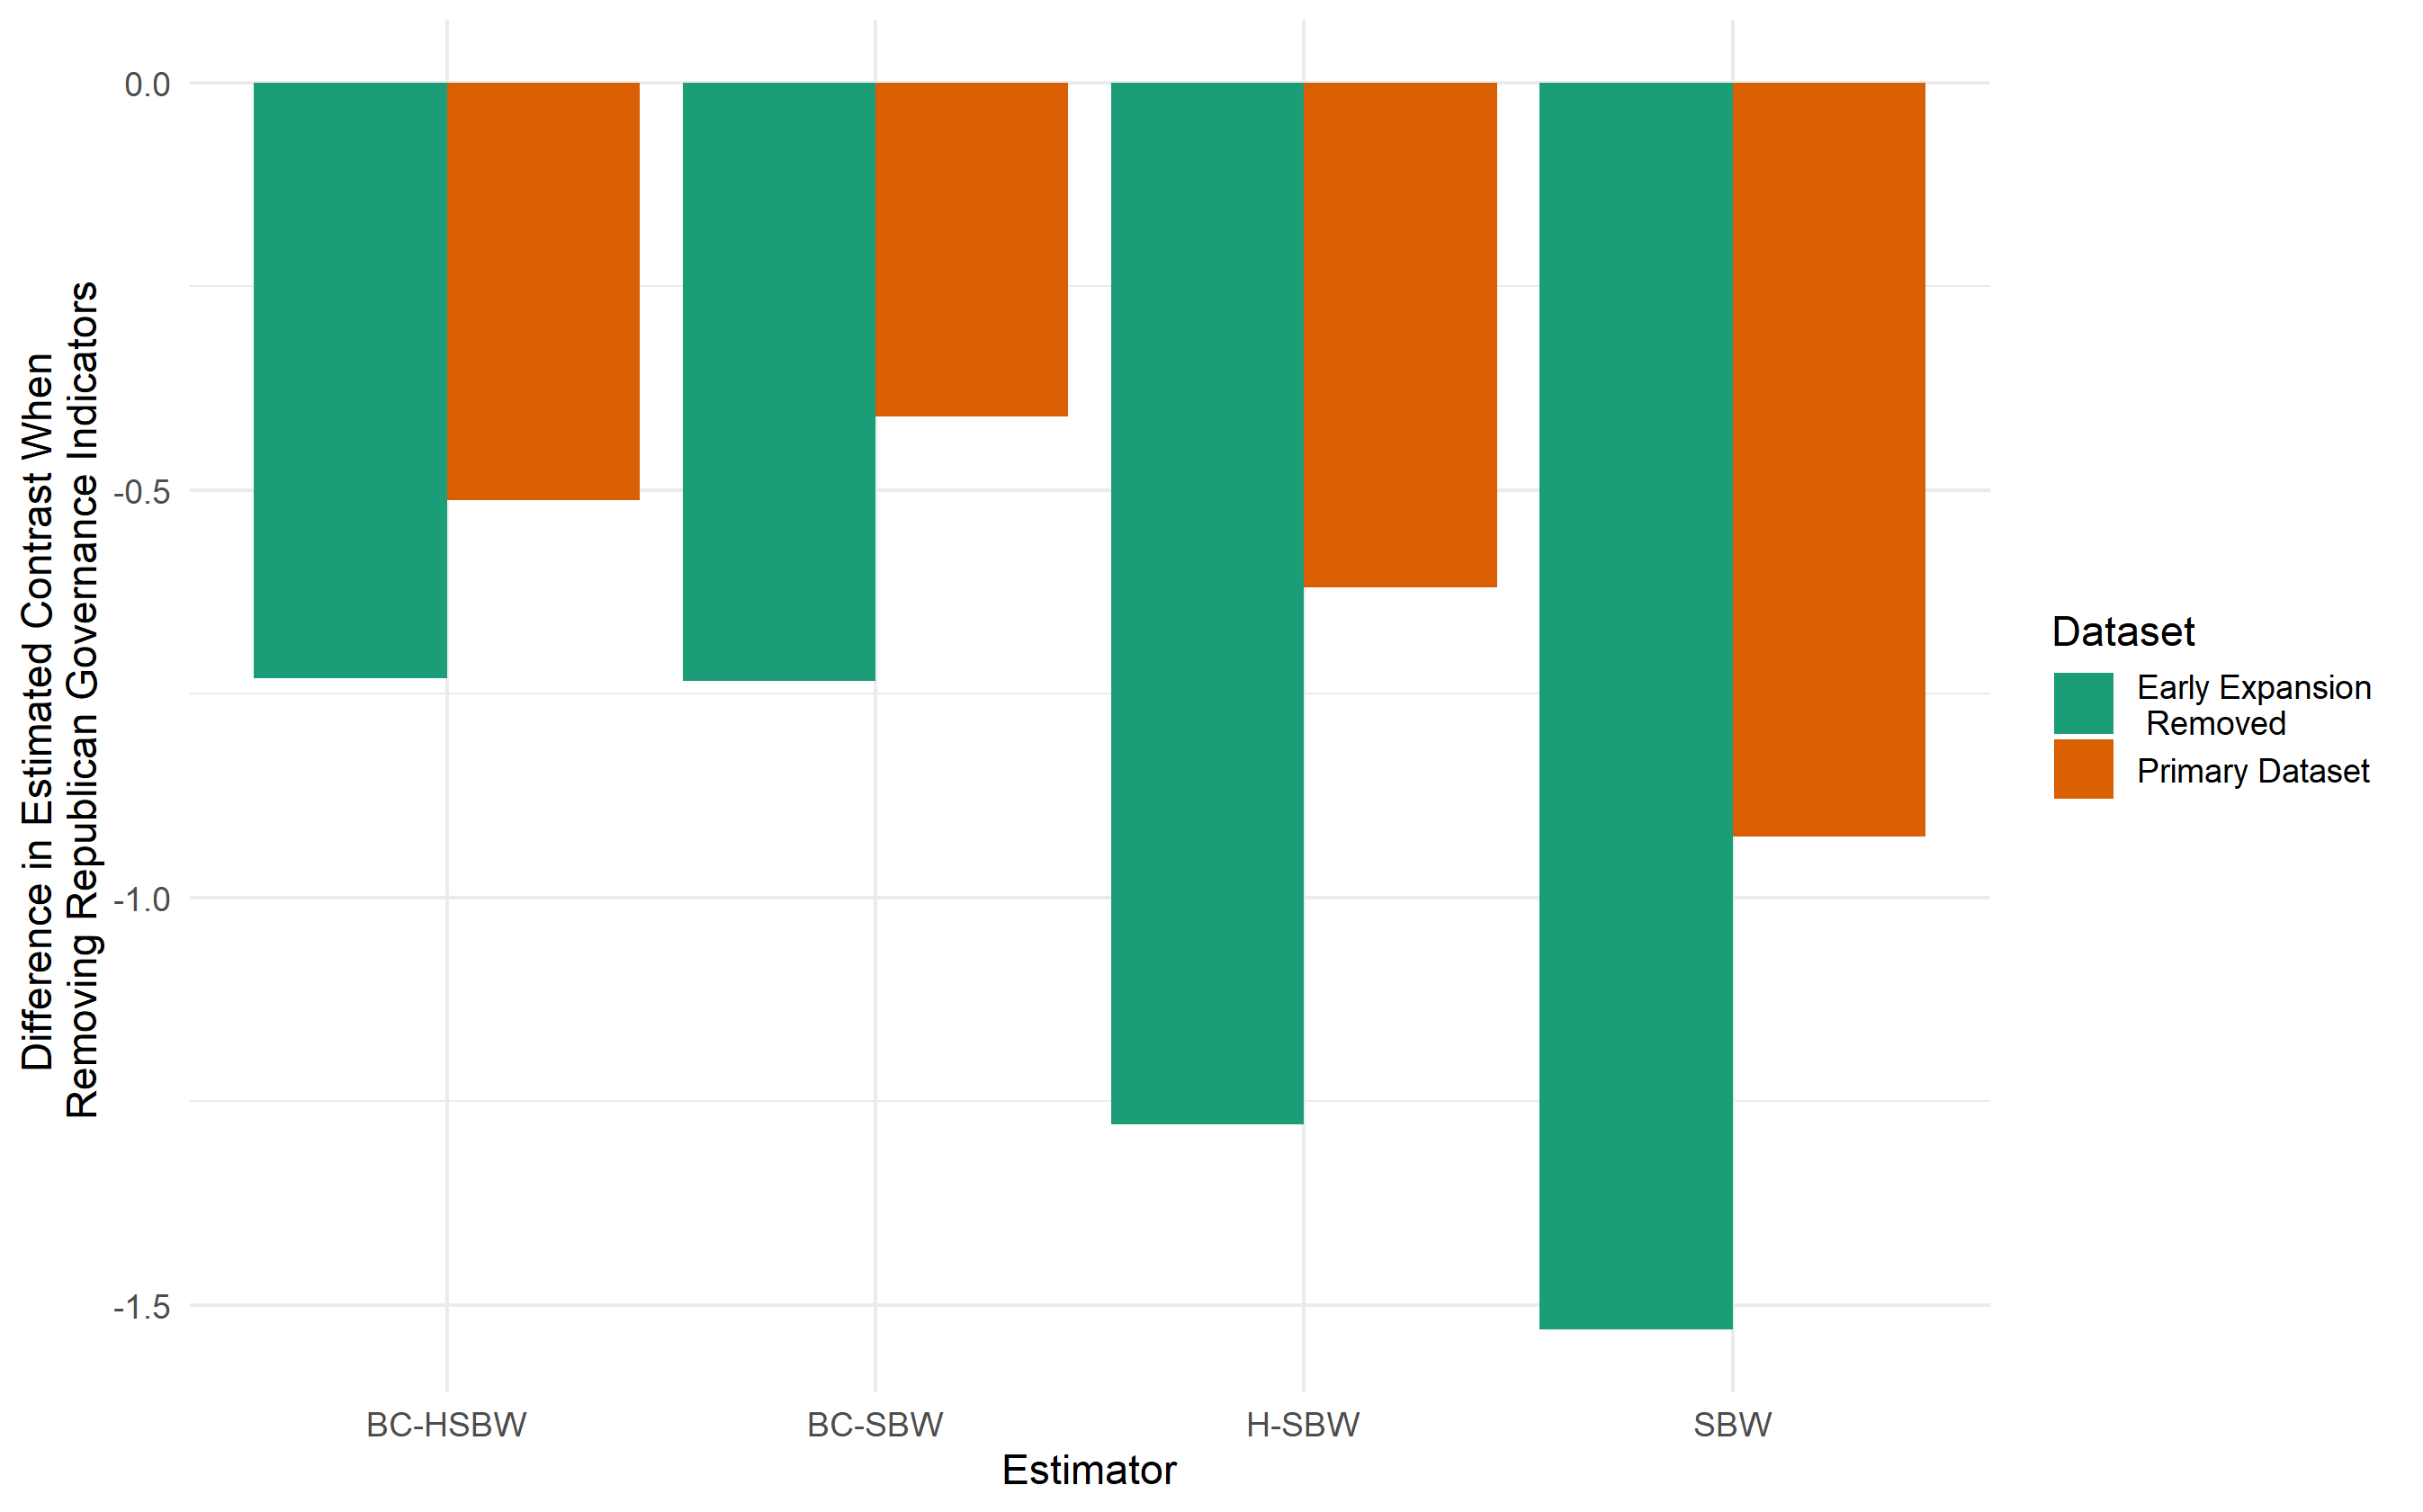
\includegraphics[scale=0.5]{01_Plots/repub-diff-c1c2.png}
    \end{center}
\end{frame}

\subsection{Sensitivity Analysis: OATE}

\begin{frame}{Robustness Check: OATE}
    \begin{itemize}
        \item What if we target a different causal estimand? \bigskip
        \item OATE is data-dependent treatment effect defined where there is sufficient overlap to estimate this difference \bigskip
        \item Logistic regression weights to find a region where the means of the covariates are balanced \bigskip
    \end{itemize}
\end{frame}

\begin{frame}{OATE weights by state: Preferred}
    \begin{center}
	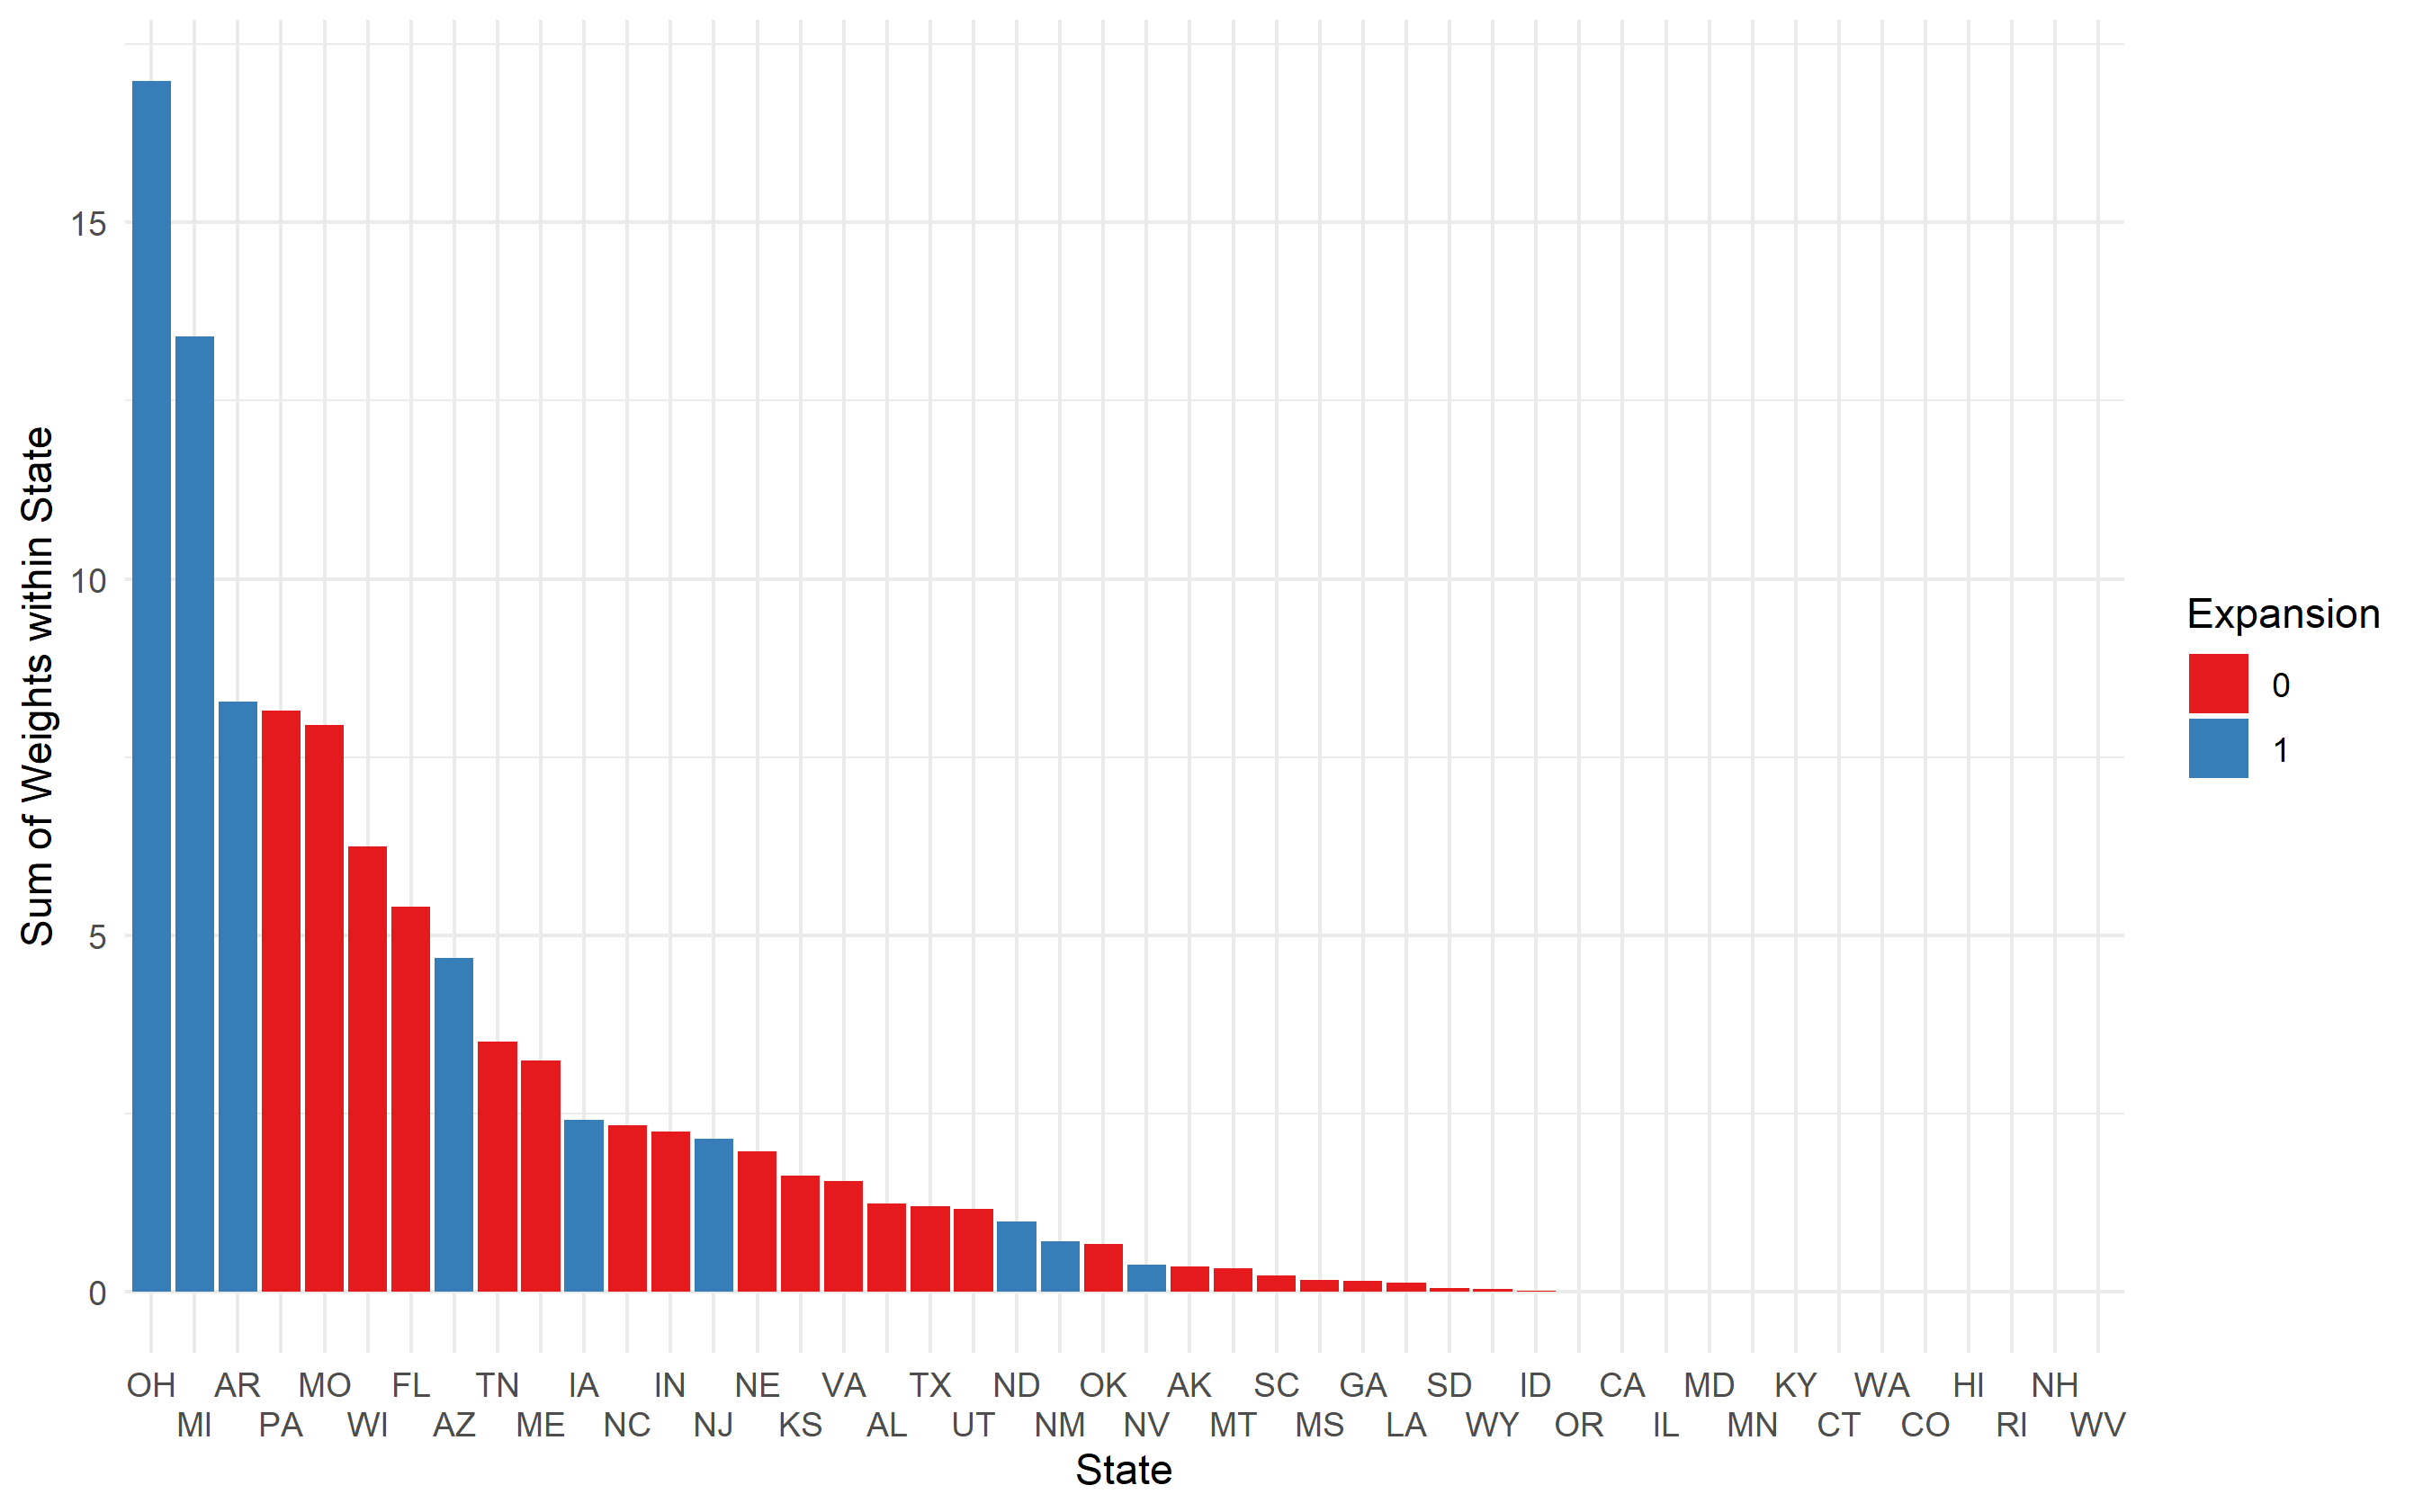
\includegraphics[scale=0.5]{01_Plots/oate-region-c1-a.png}
    \end{center}
\end{frame}

\begin{frame}{OATE region}
    \begin{itemize}
        \item Preferred dataset: \bigskip
        \begin{itemize}
            \item Mean L1 distance from control region: 2.92 \bigskip
            \item Mean L1 distance from treated region: 7.80 \bigskip
        \end{itemize}
        \item Early expansion excluded: \bigskip
        \begin{itemize}
            \item Mean L1 distance from control region: 2.94 \bigskip
            \item Mean L1 distance from treated region: 5.30 \bigskip
        \end{itemize}
    \end{itemize}
\end{frame}

\begin{frame}{OATE estimates}
\begin{table}[ht]
\centering
\begin{tabular}{rllll}
  \toprule
Psihat & Sigma estimate & Dataset & CI (states) \\ 
  \midrule
  -1.64 & sigma\_uu\_i & c1 & (-2.40, -0.89) \\ 
  -1.58 & sigma\_avg & c1 & (-2.17, -1.00) \\ 
  -1.80 & sigma\_zero & c1 & (-2.49, -1.10) \\ 
  -1.73 & sigma\_uu\_i & c2 & (-2.70, -0.76) \\ 
  -1.76 & sigma\_avg & c2 & (-2.53, -0.99) \\ 
  -1.95 & sigma\_zero & c2 & (-2.65, -1.25) \\ 
   \bottomrule
\end{tabular}
\caption{OATE results inference}
\label{tab:oateconfint}
\end{table}
\end{frame}

\begin{frame}{OATE $\Delta$}
\begin{table}[ht]
\centering
\begin{tabular}{llrll}
  \toprule
Sigma estimate & Dataset & Difference & 95 Percent CI\\ 
  \midrule
  sigma\_uu\_i & c1 & -0.96 & (-1.10, -0.81) \\ 
  sigma\_uu\_i & c2 & -0.62 & (-0.78, -0.46) \\ 
  sigma\_avg & c1 & -1.04 & (-1.19, -0.89) \\ 
  sigma\_avg & c2 & -0.64 & (-0.80, -0.48) \\ 
  sigma\_zero & c1 & -0.75 & (-0.88, -0.63) \\ 
  sigma\_zero & c2 & -0.56 & (-0.69, -0.43) \\ 
   \bottomrule
\end{tabular}
\caption{OATE differences in estimate, with and without Republican governance indicators}
\label{tab:oaterepubdiff}
\end{table}
\end{frame}

\section{Discussion}

\subsection{Discussion}

\begin{frame}{Discussion}
\begin{itemize}
    \item Propose an extension to synthetic controls/balancing weights literature to estimate the ETC with hierarchical data, measurement error in covariates \bigskip
    \item Estimate that had non-expansion states expanded Medicaid in 2014, uninsurance rates would have decreased by 2.00 percentage points (1.23, 2.82) \bigskip
    \item We show that factors associated with Republican governance are consistently associated with reducing the absolute magnitude of the estimated effects
\end{itemize}
\end{frame}

\begin{frame}{Policy implications}
    \begin{itemize}
        \item We cannot simply use existing estimates of the ETT to assume we know the ETC \bigskip
        \item Effects mediated primarily through decreasing the uninsurance rate would be smaller in absolute magnitude among states that did not expand Medicaid (see, eg, \cite{wherry2016early}) \bigskip
        \item If the goal of Medicaid expansion is decreasing uninsurance rate, should consider ways to make it easier to enroll (eg automatic enrollment based on eligibility)
    \end{itemize}
\end{frame}

\subsection{Conclusion}
\begin{frame}{Conclusion}
\begin{center}
Thank you for listening! \\ 
\newline Any questions?
\end{center}
\end{frame}


\end{document}
